%Version 3.1 December 2024
% See section 11 of the User Manual for version history
%
%%%%%%%%%%%%%%%%%%%%%%%%%%%%%%%%%%%%%%%%%%%%%%%%%%%%%%%%%%%%%%%%%%%%%%
%%                                                                 %%
%% Please do not use \input{...} to include other tex files.       %%
%% Submit your LaTeX manuscript as one .tex document.              %%
%%                                                                 %%
%% All additional figures and files should be attached             %%
%% separately and not embedded in the \TeX\ document itself.       %%
%%                                                                 %%
%%%%%%%%%%%%%%%%%%%%%%%%%%%%%%%%%%%%%%%%%%%%%%%%%%%%%%%%%%%%%%%%%%%%%

\documentclass[pdflatex,sn-mathphys-num]{sn-jnl}%

%%%% Standard Packages
\usepackage{graphicx}%
\usepackage{multirow}%
\usepackage{amsmath,amssymb,amsfonts}%
\usepackage{amsthm}%
\usepackage{mathrsfs}%
\usepackage[title]{appendix}%
\usepackage{xcolor}%
\usepackage{textcomp}%
\usepackage{manyfoot}%
\usepackage{booktabs}%
\usepackage{algorithm}%
\usepackage{algorithmicx}%
\usepackage{algpseudocode}%
\usepackage{listings}%
\usepackage{subcaption}%
\usepackage{array}%
\usepackage{placeins}%
\usepackage{claims}%
\showclaimsfalse
% Generated by oran_causal.analysis.paper_values from spec/values.toml and data/records.
% Do not edit: run `uv run python -m oran_causal.analysis.paper_values`.
\defval{appa.prior.directed}{33}
\defval{br.pcorr_eq.recall}{0.72}
\defval{br.pcorr_native.recall}{0.69}
\defval{s1.attr.declared}{13}
\defval{s1.attr.true}{12}
\defval{s1.ex.confirmed}{26}
\defval{s1.ex.n_exists}{43}
\defval{s1.far.total}{20}
\defval{s1.far.true}{8}
\defval{s1.gt.dbl.int.prec}{0.88}
\defval{s1.gt.dbl.int.rec}{0.35}
\defval{s1.gt.dbl.pmrt.prec}{0.59}
\defval{s1.gt.dbl.pmrt.rec}{0.80}
\defval{s1.gt.dbl.qacm.prec}{0.80}
\defval{s1.gt.dbl.qacm.rec}{0.40}
\defval{s1.gt.dbl.shap.prec}{0.75}
\defval{s1.gt.dbl.shap.rec}{0.60}
\defval{s1.gt.dbl.tt.prec}{0.83}
\defval{s1.gt.dbl.tt.rec}{0.25}
\defval{s1.gt.episodes}{40}
\defval{s1.gt.half.prec}{1.00}
\defval{s1.gt.hypotheses}{60}
\defval{s1.k0.binom_level}{0.01}
\defval{s1.k0.binom_tail}{0.03}
\defval{s1.k0.m}{60}
\defval{s1.k0.n_reject}{7}
\defval{s1.k0.tail3}{0.030}
\defval{s1.k0n.fam_max}{0.060}
\defval{s1.k0n.fam_min}{0.047}
\defval{s1.k0n.rate}{0.053}
\defval{s1.map.corr.placebo}{3}
\defval{s1.map.corr.prec}{0.86}
\defval{s1.map.corr.rec}{0.21}
\defval{s1.map.corr.wrong}{1}
\defval{s1.map.gby.placebo}{13}
\defval{s1.map.gby.prec}{0.59}
\defval{s1.map.gby.rec}{0.76}
\defval{s1.map.gby.wrong}{6}
\defval{s1.map.gr.placebo}{1}
\defval{s1.map.gr.prec}{0.69}
\defval{s1.map.gr.rec}{0.62}
\defval{s1.map.gr.wrong}{4}
\defval{s1.map.int.placebo}{6}
\defval{s1.map.int.prec}{0.88}
\defval{s1.map.int.rec}{0.24}
\defval{s1.map.int.wrong}{0}
\defval{s1.map.pmrt.placebo}{0}
\defval{s1.map.pmrt.prec}{0.92}
\defval{s1.map.pmrt.rec}{0.79}
\defval{s1.map.pmrt.wrong}{0}
\defval{s1.map.qacm.placebo}{5}
\defval{s1.map.qacm.prec}{0.89}
\defval{s1.map.qacm.rec}{0.28}
\defval{s1.map.qacm.wrong}{0}
\defval{s1.map.shap.placebo}{8}
\defval{s1.map.shap.prec}{0.93}
\defval{s1.map.shap.rec}{0.48}
\defval{s1.map.shap.wrong}{0}
\defval{s1.map.tt.placebo}{6}
\defval{s1.map.tt.prec}{1.00}
\defval{s1.map.tt.rec}{0.21}
\defval{s1.map.tt.wrong}{1}
\defval{s1.null.ci.hi}{0.29}
\defval{s1.null.ci.lo}{0.043}
\defval{s1.null.count}{21}
\defval{s1.null.open.ci.hi}{0.16}
\defval{s1.null.open.ci.lo}{0.017}
\defval{s1.null.open.count}{12}
\defval{s1.null.open.rate}{0.075}
\defval{s1.null.rate}{0.15}
\defval{s1.p2.gby.wins120}{4}
\defval{s1.p2.gby.wins60}{2}
\defval{s1.p2.n120}{5}
\defval{s1.p2.n60}{10}
\defval{s1.placebo.granger_by}{13}
\defval{s1.pmrt.declared}{28}
\defval{s1.pmrt.indet}{3}
\defval{s1.pmrt.precision}{0.92}
\defval{s1.pmrt.recall}{0.79}
\defval{s2.assoc.ratio_max}{5.4}
\defval{s2.assoc.ratio_min}{4.5}
\defval{s2.attr.declared}{7}
\defval{s2.dec.aa.dn}{-0.22}
\defval{s2.dec.aa.dn_hi}{-0.14}
\defval{s2.dec.aa.dn_lo}{-0.30}
\defval{s2.dec.aa.dr}{$-0.22$}
\defval{s2.dec.aa.dr_hi}{$-0.14$}
\defval{s2.dec.aa.dr_lo}{$-0.30$}
\defval{s2.dec.aa.rcv}{0.00}
\defval{s2.dec.aa.ret}{1.00}
\defval{s2.dec.aa.rlf}{1.00}
\defval{s2.dec.aa.rlf_hi}{1.00}
\defval{s2.dec.aa.rlf_lo}{1.00}
\defval{s2.dec.gt.dn}{0.02}
\defval{s2.dec.gt.dn_hi}{0.09}
\defval{s2.dec.gt.dn_lo}{-0.04}
\defval{s2.dec.gt.dr}{$+0.02$}
\defval{s2.dec.gt.dr_hi}{$0.09$}
\defval{s2.dec.gt.dr_lo}{$-0.04$}
\defval{s2.dec.gt.rcv}{0.24}
\defval{s2.dec.gt.ret}{1.32}
\defval{s2.dec.gt.rlf}{1.01}
\defval{s2.dec.gt.rlf_hi}{1.09}
\defval{s2.dec.gt.rlf_lo}{0.94}
\defval{s2.dec.ns.rcv}{0.22}
\defval{s2.dec.ns.ret}{1.18}
\defval{s2.dec.ns.rlf}{0.99}
\defval{s2.dec.ns.rlf_hi}{1.04}
\defval{s2.dec.ns.rlf_lo}{0.94}
\defval{s2.dec.pmrt.dn}{0.25}
\defval{s2.dec.pmrt.dn_hi}{0.36}
\defval{s2.dec.pmrt.dn_lo}{0.14}
\defval{s2.dec.pmrt.dr}{$+0.25$}
\defval{s2.dec.pmrt.dr_hi}{$0.36$}
\defval{s2.dec.pmrt.dr_lo}{$0.14$}
\defval{s2.dec.pmrt.rcv}{0.47}
\defval{s2.dec.pmrt.ret}{1.67}
\defval{s2.dec.pmrt.rlf}{1.31}
\defval{s2.dec.pmrt.rlf_hi}{1.56}
\defval{s2.dec.pmrt.rlf_lo}{1.10}
\defval{s2.dec.seeds}{160}
\defval{s2.defer.ptx_up.gt}{2\,370}
\defval{s2.defer.ptx_up.pmrt}{8\,674}
\defval{s2.ex.confirmed}{22}
\defval{s2.ex.n_exists}{40}
\defval{s2.far.true}{9}
\defval{s2.gt.dbl.pmrt.prec}{0.73}
\defval{s2.gt.half.prec}{1.00}
\defval{s2.k0.m}{60}
\defval{s2.k0.n_reject}{0}
\defval{s2.k0n.fam_max}{0.063}
\defval{s2.k0n.fam_min}{0.038}
\defval{s2.k0n.rate}{0.050}
\defval{s2.map.corr.placebo}{8}
\defval{s2.map.corr.prec}{0.80}
\defval{s2.map.corr.rec}{0.28}
\defval{s2.map.corr.wrong}{2}
\defval{s2.map.gby.placebo}{29}
\defval{s2.map.gby.prec}{0.54}
\defval{s2.map.gby.rec}{0.76}
\defval{s2.map.gby.wrong}{6}
\defval{s2.map.gr.placebo}{19}
\defval{s2.map.gr.prec}{0.60}
\defval{s2.map.gr.rec}{0.62}
\defval{s2.map.gr.wrong}{6}
\defval{s2.map.int.placebo}{1}
\defval{s2.map.int.prec}{0.80}
\defval{s2.map.int.rec}{0.14}
\defval{s2.map.int.wrong}{0}
\defval{s2.map.pmrt.placebo}{0}
\defval{s2.map.pmrt.prec}{0.86}
\defval{s2.map.pmrt.rec}{0.62}
\defval{s2.map.pmrt.wrong}{0}
\defval{s2.map.qacm.placebo}{0}
\defval{s2.map.qacm.prec}{0.83}
\defval{s2.map.qacm.rec}{0.17}
\defval{s2.map.qacm.wrong}{0}
\defval{s2.map.shap.placebo}{0}
\defval{s2.map.shap.prec}{0.80}
\defval{s2.map.shap.rec}{0.28}
\defval{s2.map.shap.wrong}{0}
\defval{s2.map.tt.placebo}{22}
\defval{s2.map.tt.prec}{0.63}
\defval{s2.map.tt.rec}{0.17}
\defval{s2.map.tt.wrong}{0}
\defval{s2.placebo.granger_by}{29}
\defval{s2.plc.rec_max}{0.55}
\defval{s2.pmrt.declared}{22}
\defval{s2.pmrt.indet}{1}
\defval{s2.ptx_nbr_rlf.primary_p}{0.49}
\defval{s3.dec.aa.dn}{-0.26}
\defval{s3.dec.aa.dn_hi}{-0.17}
\defval{s3.dec.aa.dn_lo}{-0.34}
\defval{s3.dec.aa.dr}{$-0.26$}
\defval{s3.dec.aa.dr_hi}{$-0.17$}
\defval{s3.dec.aa.dr_lo}{$-0.34$}
\defval{s3.dec.aa.rcv}{0.00}
\defval{s3.dec.aa.ret}{1.00}
\defval{s3.dec.aa.rlf}{1.00}
\defval{s3.dec.aa.rlf_hi}{1.00}
\defval{s3.dec.aa.rlf_lo}{1.00}
\defval{s3.dec.gt.dn}{-0.04}
\defval{s3.dec.gt.dn_hi}{0.03}
\defval{s3.dec.gt.dn_lo}{-0.10}
\defval{s3.dec.gt.dr}{$-0.04$}
\defval{s3.dec.gt.dr_hi}{$0.03$}
\defval{s3.dec.gt.dr_lo}{$-0.10$}
\defval{s3.dec.gt.rcv}{0.22}
\defval{s3.dec.gt.ret}{1.29}
\defval{s3.dec.gt.rlf}{0.94}
\defval{s3.dec.gt.rlf_hi}{0.97}
\defval{s3.dec.gt.rlf_lo}{0.90}
\defval{s3.dec.ns.rcv}{0.26}
\defval{s3.dec.ns.ret}{1.15}
\defval{s3.dec.ns.rlf}{0.96}
\defval{s3.dec.ns.rlf_hi}{0.99}
\defval{s3.dec.ns.rlf_lo}{0.93}
\defval{s3.dec.pmrt.dn}{0.00}
\defval{s3.dec.pmrt.dn_hi}{0.00}
\defval{s3.dec.pmrt.dn_lo}{0.00}
\defval{s3.dec.pmrt.dr}{$0.00$}
\defval{s3.dec.pmrt.dr_hi}{$0.00$}
\defval{s3.dec.pmrt.dr_lo}{$0.00$}
\defval{s3.dec.pmrt.rcv}{0.26}
\defval{s3.dec.pmrt.ret}{1.15}
\defval{s3.dec.pmrt.rlf}{0.96}
\defval{s3.dec.pmrt.rlf_hi}{0.99}
\defval{s3.dec.pmrt.rlf_lo}{0.93}
\defval{s3.dec.seeds}{160}
\defval{s3.gate.dev_episodes}{40}
\defval{s3.gate.g_rlf}{35.025}
\defval{s3.gate.g_v}{19\,953.65}
\defval{s3.mgpmrt.dr}{$-0.06$}
\defval{s3.mgpmrt.rlf}{1.05}
\defval{s4.c1.r2_max}{0.94}
\defval{s4.c1.r2_min}{0.33}
\defval{s4.cdl.conditions}{30}
\defval{s4.cdl.invalid}{9}
\defval{s4.conf.corr_all}{0.77}
\defval{s4.conf.corr_min}{1.00}
\defval{s4.conf.gbm_max}{0.06}
\defval{s4.conf.gbm_min}{0.02}
\defval{s4.conf.pcorr_all}{0.056}
\defval{s4.conf.rcot2_all}{0.23}
\defval{s4.dither.max}{0.054}
\defval{s4.dither.min}{0.042}
\defval{s4.e4.pcorr_eq.recall_24k}{0.90}
\defval{s4.e4.pmrtgbm.recall_max}{0.075}
\defval{x11.delta_dbl.changed}{16}
\defval{x11.delta_half.changed}{10}
\defval{x11.other.changed_max}{2}
\defval{x11.pmrt.sign_acc_min}{1.00}
\defval{x14.gby.wrong_s1}{24}
\defval{x14.gby.wrong_s2}{21}
\defval{x15.block_diff}{0.30}
\defval{x15.p.never_sleep}{0.17}
\defval{x15.p.noarb}{0.15}
\defval{x15.perm_p}{0.009}
\defval{x15.pooled.dr}{0.10}
\defval{x15.pooled.rlf}{1.18}
\defval{x15.r.never_sleep_s2}{0.22}
\defval{x15.r.never_sleep_s3}{0.26}
\defval{x15.rej.s2}{0.37}
\defval{x15.rej.s3}{0.35}
\defval{x15.sd.s2}{0.85}
\defval{x15.sd.s3}{1.1}
\defval{x15.trim.s2}{0.21}
\defval{x15.trim.s3}{0.041}
\defval{x16.gate.median_pct}{3.5}
\defval{x16.map.rel_max}{$+6.5$}
\defval{x16.map.rel_min}{$-2.9$}
\defval{x8.lim.1e3}{2 \times 10^{-3}}
\defval{x8.lim.2e4}{6 \times 10^{-4}}
\defval{x8.n_variants}{590}
\defval{x8.redraws}{9\,999}
\defval{x8.share.1e3}{7.9 \times 10^{-4}}
\defval{x8.share.2e4}{1.1 \times 10^{-4}}
\defval{x8.tol_pct}{7.5}
\defval{x8.variants_with_decl}{2}

%%%%

\theoremstyle{thmstyleone}%
\newtheorem{theorem}{Theorem}%
\newtheorem{proposition}[theorem]{Proposition}%
\newtheorem{corollary}{Corollary}%
\newtheorem{lemma}{Lemma}%

\theoremstyle{thmstyletwo}%
\newtheorem{example}{Example}%
\newtheorem{remark}{Remark}%

\theoremstyle{thmstylethree}%
\newtheorem{definition}{Definition}%

\raggedbottom

\usepackage{accsupp}
\ExplSyntaxOn
\cs_new_protected:Npn \cdd_verdict:nn #1#2
  { \BeginAccSupp { ActualText = {#1} } \textsc {#2} \EndAccSupp { } }
\NewDocumentCommand \verdict { m } { \exp_args:Nee \cdd_verdict:nn { \str_uppercase:n {#1} } {#1} }
\ExplSyntaxOff
\begin{document}

\title[Design-Based Causal Effect Maps for xApp Conflicts]{Design-Based Causal Effect Maps for O-RAN xApp Conflicts}

\author*[1]{\fnm{First} \sur{Author}}\email{first.author@example.com}

\author[1]{\fnm{Second} \sur{Author}}\email{second.author@example.com}

\author[2]{\fnm{Third} \sur{Author}}\email{third.author@example.com}

\affil*[1]{\orgdiv{Department}, \orgname{Organization}, \orgaddress{\city{City}, \country{Country}}}

\affil[2]{\orgdiv{Department}, \orgname{Organization}, \orgaddress{\city{City}, \country{Country}}}

\abstract{In Open Radio Access Networks (O-RAN), xApps from different vendors can conflict even when each controls a
different parameter, because the parameters act on the same key performance indicators (KPIs). Resolving such
conflicts requires knowing which parameter moves which KPI, and in which direction. The logs that could reveal this
are written by controllers that react to the same network state that drives the KPIs, so relationships learned from
them are confounded. In this work, we propose randomising the conflict-mitigation layer's accept-or-reject decisions
and logging their probabilities, and introduce the predictable matched-filter randomisation test (PMRT), which redraws
these decisions to test the sharp null that a parameter family never changes a KPI. Its false discovery rate control
is asymptotic, needs no network model, and covers these nulls but not effect signs or the cells that carry an effect.
In one simulated scenario, PMRT declared nothing on placebo logs and no wrong-sign edge. Its precision against a
simulated ground truth, \val{s1.map.pmrt.prec} on randomised and \val{s2.map.pmrt.prec} on confounded logs, fell to \val{s1.gt.dbl.pmrt.prec} and \val{s2.gt.dbl.pmrt.prec} under a doubled
materiality threshold. A referee acting on the map alone breached a radio-link-failure guard. Behind an
edge-certification gate, the referee met every guard and matched the best static rule, which never lets a pico cell
sleep, and even the ground-truth map did no better. Randomised logging thus supports valid discovery, and the decision
study locates the remaining limit of safe mitigation in the guards rather than in the map.}

\keywords{O-RAN, xApp conflict mitigation, causal discovery, randomisation inference, design-based inference, near-RT RIC}

\maketitle

\section{Introduction}
\label{sec:introduction}

In an Open Radio Access Network (O-RAN), applications from different vendors, the xApps, run on the near-real-time
radio access network (RAN) Intelligent Controller (near-RT RIC) and adjust the control parameters of the same cells,
often with conflicting objectives. The conflict mitigation report of O-RAN Working Group~3 distinguishes three types
of conflict~\cite{ORANConflictMit} (Figure~\ref{fig:intro_conflict}). In a direct conflict two xApps write the same
parameter, as when an energy-saving (ES) xApp lowers the transmit power that a coverage and capacity optimisation
(CCO) xApp sets high~\cite{QACM2024}. In an indirect conflict they write different parameters that act on the same
key performance indicator (KPI), as when mobility robustness optimisation (MRO) and mobility load balancing (MLB) both
move the handover boundary~\cite{ORANConflictMit,wadud2025mobility}. In an implicit conflict, finally, the coupling
runs through the network without any shared parameter. Indirect and implicit conflicts are the harder to detect, since
neither request reveals the interaction, and resolving them requires a map of which control parameter moves which
KPI, and in which direction.

\begin{figure}[b]
\centering
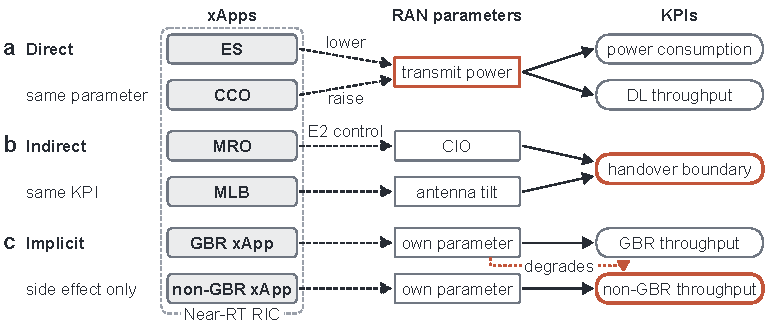
\includegraphics[width=\textwidth]{figures/fig_conflict_types.pdf}
\caption{O-RAN conflict types.}
\label{fig:intro_conflict}
\end{figure}

A growing literature learns such maps from network
data~\cite{QACM2024,PACIFISTA,Sharma_2025,santos2026conflictairan}, but these data are logs written by the controllers
themselves. An xApp issues a request because of the state of its cell, and the same state drives the KPIs, so an
association between requests and KPIs mixes the effect of the request with the controller's reaction to the network.
Relationships learned from such logs are therefore confounded, and a discovery method can report effects where none
exist; in our evaluation, every associational baseline reported edges on placebo logs, in which no parameter has any
effect.

This confounding can be removed within the near-RT RIC itself. Every xApp request already passes through the
conflict-mitigation layer of the RIC, which accepts or rejects it~\cite{ORANRICARCH}, and we call the rule that makes
this choice the referee. If the referee draws each decision at random with a probability that it records, the logs
carry a known experimental design, and redrawing the logged decisions yields a randomisation test of whether a
parameter affects a KPI. Such a test is design-based: its validity rests on the randomisation performed by the
referee rather than on a model of the network, at the cost of rejecting some requests at random while the logs are
collected. We evaluate this approach on three questions: whether a design-based test is valid on such logs, whether
the causal map it learns agrees with an independent ground truth, and whether decisions taken with the map improve on
static rules within the safety limits. The evaluation uses a system-level simulation of an O-RAN surge scenario, in
which energy-saving xApps conflict with a slice-protection xApp, and controlled environments with known causal
structure.

The first two answers are positive. The test declared no effect on placebo logs and never reported an effect with the
wrong sign, and most of the effects it reported were confirmed by a knockout ground truth, on randomised and
confounded logs alike. In the controlled environments, tests that ignored the logging design lost their error control
once the logging followed a dithered setpoint instead of independent draws, whereas tests that used the design kept
it. The third answer is negative: a referee acting on the map reduced protected-slice violations but breached a
radio-link-failure limit, and behind a gate that admits only certified-safe rejections it fell back to the best static
rule, as did the true causal map. In this scenario, the safety guards rather than knowledge of the network limit what
conflict mitigation can achieve.

The paper makes three contributions.
\begin{enumerate}
\item \textbf{The test}. PMRT, a design-based test that learns signed causal effect maps from near-RT RIC request
logs with logged probabilities, with an explicit estimand and the conditions for its asymptotic validity.
\item \textbf{The validity evidence}. Placebo and null-outcome checks on the simulator, and a study on five
controlled environments of whether edge tests keep their error rate when the logging design is known. The evidence
suggests a practical placebo check, a necessary condition only, for learned discovery pipelines on designed logs.
\item \textbf{The decision study}. A test of whether such a map improves safe decisions, with a map-driven referee
and an edge-certification gate. In the evaluated scenario the map gave no such improvement, and this gap between a
valid map and a better safe policy is the paper's central result.
\end{enumerate}
The work builds on our conference paper on causal discovery-driven conflict mitigation, CDD
O-RAN~\cite{dahal2026cddoran}, but replaces its method rather than extending it.

% Step 5 rewrite (2026-10-14): Background and Related Work. Subsections and table kept (user); gap labels G1-G3
% removed from print; table cut to five columns with short cells and one note; formal subsection titles.
\section{Background and related work}
\label{sec:related}

% Section 2 rewritten 2026-10-11 (W5) to outline v2 (s.2) and decision D8: three gaps, one comparison table (W4 draft
% reviews/2026-10-10/drafts/related_work_table.tex, replacing the pre-v2 Table 1). Sources: RWS =
% reviews/2026-10-10/drafts/related_work_sources.md (W4; bibliographic data checked against Crossref / arXiv records;
% one-sentence content from the abstracts); prior-method facts already in the pre-v2 Sections 1-2 keep their checks
% against archive/reference-papers (full texts, 2026-10-09). Sources marked "(content from prior knowledge)" in RWS
% are cited only for what their titles say. TERM = TERMINOLOGY.md.

This section reviews prior work in three areas: causal inference from logged data, the learning of conflict maps
in O-RAN, and safe conflict mitigation. Table~\ref{tab:related} summarises the method families of each area and
positions the proposed approach among them. % src: outline v2 s.2 (G1-G3); PAPER_PLAN.md D8; RWS (rows F1-F11)

\subsection{Causal effects from feedback-driven logs}
\label{sec:related_design}

When a controller produced the logs, an edge test draws its validity either from assumptions about the
data-generating process or from a known assignment mechanism. RIC logs leave the assumptions untestable, because
requests react to the state that drives the KPIs, and no O-RAN work we found takes the mechanism from the RIC's own
decisions. % src: RWS G1 (F7 model-based, F8 design-based); outline v2 s.2.1 (gap); P2b s.1 (no rhetorical question)
Observational causal discovery rests on the first kind. Granger causality~\cite{granger1969causal} and the
Peter--Clark (PC) algorithm~\cite{spirtes2000causation} assume that no common cause goes unmeasured, NOTEARS fits an
acyclic structural equation model~\cite{zheng2018notears}, and the randomized conditional correlation test
(RCoT)~\cite{strobl2019rcot} and PCMCI~\cite{runge2019pcmci} test conditional independence. % src: RWS G1 (granger1969causal, spirtes2000causation: causal sufficiency; zheng2018notears, strobl2019rcot, runge2019pcmci abstracts); W16 P2b (merged)

Design-based inference takes its validity from the assignment mechanism instead: when the assignment probabilities
are known, redrawing the assignments under a sharp null, which states that the assignment changes no unit's outcome, gives a
p-value with no model of the
outcomes~\cite{imbens2015causal}. % src: RWS G1 (imbens2015causal); pre-v2 Section 2.1
Such tests reach sequential experiments on a single time series~\cite{bojinov2019timeseries}, switchback
experiments~\cite{bojinov2023switchback} and response-adaptive designs, where re-running the adaptive assignment rule
keeps the type I error only under conditions~\cite{simon2011randomization}. The conditional randomisation test keeps any test statistic
valid~\cite{candes2018knockoffs}, and Benjamini--Yekutieli (BY) control keeps the FDR of many tests
under arbitrary dependence~\cite{benjamini2001dependency}. % src: RWS G1 (bojinov2019timeseries abstract; bojinov2023switchback abstract: exact randomisation p-values, checked 2026-10-13; candes2018knockoffs, benjamini2001dependency); W16 P2b (shortened)
Under known interference, design-based estimators~\cite{aronow2017interference} and randomisation
tests~\cite{basse2019interference} also exist. In networks, A/B tests of congestion
control are biased when the arms share a bottleneck~\cite{spang2021unbiased}, and CausalSim uses randomised trial
data to debias network traces~\cite{alomar2023causalsim}. % src: RWS G1 (aronow2017interference: estimators and variance bounds; basse2019interference: tests; spang2021unbiased, alomar2023causalsim abstracts); reference audit 2026-10-13 (kohavi2009controlled dropped)
Off-policy evaluation reweights logged rewards by the logged action probabilities, with doubly robust
variants~\cite{dudik2014doubly} and intervals and M-estimation under adaptive logging~\cite{hadad2021adaptive,zhang2021mestimators}, but it estimates the
value of a policy, not the edges of a map. % src: Dudik et al. abstract and s. 2-3; RWS G1 (hadad2021adaptive title); RWS positioning (F10 estimates policy values, not edges)
% W20: moved here from the end of the CDD O-RAN paragraph, so that "these" cannot be read as CDD O-RAN (P4 s.1).
These methods come from designed or bandit experiments, and none tests a signed map of many edges under a
state-dependent policy. % src: RWS positioning (G1); outline v2 s.2.1 (gap); RWS (search for O-RAN causal discovery found none)

Our conference work, CDD O-RAN, avoided confounding with an offline exploration phase in which a random policy
perturbed every control parameter~\cite{dahal2026cddoran}. It kept each edge whose smoothed conditional mutual
information (CMI) exceeded a threshold, so its graph was unsigned and without error control. % src: archive/xApp-Nana-Conference-2026/sections/03_proposed_method.tex (deployment model; CMI edge discovery, EMA, threshold); advisor 2026-10-09 (CDD O-RAN limits); TERM s.12 D5 (never "invalid")
The present method draws its identification from operational accept-or-reject decisions
instead. % src: TERM Paper identity (never "extension"); outline v2 s.2 (positioning sentence); W16 P2b (shortened)

\subsection{Conflict maps in O-RAN}
\label{sec:related_maps}

Existing conflict maps mostly predict KPIs or explain a fitted model. None that we found declares signed,
error-controlled effects of actions from logs whose actions the controller itself chose, and the one causal approach
relies on a correct graph with every confounder measured. % src: RWS positioning (G2: F2 and F4 associations or attributions; F5 model-based); outline v2 s.2.2; P2b s.1
Shapley additive explanations (SHAP) attribute a model's prediction to its inputs~\cite{lundberg2017shap}, and
their tree form~\cite{lundberg2020trees} underlies our SHAP-GBDT baseline on gradient-boosted decision trees (GBDT). % W16 P2b: "make no causal claim by themselves" cut (the opener says it). src: RWS G2 (lundberg2017shap, lundberg2020trees); CDD-ORAN/cdd_oran/decision/baselines_disc.py docstring (HistGBDT + shap.TreeExplainer)
In O-RAN, EXPLORA links a reinforcement-learning agent's actions to attributes of its input
state~\cite{fiandrino2023explora}, and a survey covers explainable artificial intelligence for O-RAN
control~\cite{brik2025xai}. % src: RWS G2 (fiandrino2023explora, brik2025xai abstracts)
% W16 P2b: "Such attributions describe a fitted model, not the effect of an action" cut (restated the opener).

% W16 P2b: "Conflict detectors differ mainly in where they get the knowledge of which parameter affects which KPI." cut.
Rule-based conflict detectors take parameter groups configured by the operator~\cite{adamczyk2023conflict} or derived from
conflict graphs~\cite{wadud2025mobility}. % src: Adamczyk s. III-C; Wadud abstract, Algorithm 1
Learned detectors use a graph convolutional network trained on synthetic data~\cite{alshami2026conflict}, GraphSAGE
reconstructions of conflict graphs~\cite{zolghadr2025conflict} or a two-tower encoder of a sparse parameter-KPI
graph~\cite{santos2026conflictairan}, the last two trained on data from a known conflict model. % src: Al Shami arXiv v3 abstract; Zolghadr arXiv abstract; Two-tower.md (abstract, s. I, s. IV)
XAI4C adds explainability-based detection and mitigation to the near-RT RIC~\cite{varshney2025xai4c}, and PACIFISTA
profiles each application in a sandbox to rate conflicts before deployment~\cite{PACIFISTA}. % src: RWS G2 (varshney2025xai4c abstract); PACIFISTA abstract, Conclusions
% W16 P2b: "All of them identify interactions by the fit of a learned model ..." cut (restated the opener).
Sharma et al.\ go further: they assemble a causal directed acyclic graph (DAG) from a SHAP analysis and estimate signed
average treatment effects, with refutation tests~\cite{Sharma_2025}. Their estimates are identified only if that
graph is correct and no confounder is left unmeasured. Our SHAP-GBDT baseline keeps only their importance step. % src: Sharma s. IV-V; BD docstring (shap_gbdt); advisor 2026-10-09 (qualifier)

\subsection{Safe conflict mitigation}
\label{sec:related_decisions}

Mitigation in the RIC takes the parameter-to-KPI relations as given or learns predictors of KPI levels. Safety
guarantees come from data on a whole policy or from a model of the system. None certifies decisions from the
uncertainty of a causal effect map. % src: advisor 2026-10-09 (positioning); RWS positioning (G3); outline v2 s.2.3 (gap); P2b s.1
Once a conflict is found, mitigation decides what to apply~\cite{ORANConflictMit,polese2023oran}: the framework of
Adamczyk and Kliks gives priority to one of the conflicting xApps~\cite{adamczyk2023conflict}. % src: pre-v2 Section 2.3; RWS G3 (polese2023oran: context); Adamczyk s. IV
Quality-of-service-aware conflict mitigation (QACM) picks the configuration that satisfies the most xApps, using
regression predictors of their KPIs~\cite{QACM2024}, and Wadud et al.\ compared it with priority and reset rules on a
direct transmit-power conflict~\cite{wadud2025mobility}. % src: QACM abstract, s. IV-B; Wadud s. V (NC, SBD, P-ES, P-MRO, QACM; direct conflict over TXP)
Other layers let two xApps learn as a team~\cite{iturria2022matl}, train a scheduler that selects which xApps
act~\cite{cinemre2026scheduler}, or test conflicting actions in a network digital twin before applying
them~\cite{giannopoulos2025comix}. % src: RWS G3 (iturria2022matl abstract); Cinemre arXiv v3 abstract; COMIX arXiv abstract

Safe reinforcement learning (RL) keeps a learning controller away from harmful actions~\cite{gu2024safereview},
for example by shielding~\cite{alshiekh2018shield}, and in RAN slicing its safety has been
shown empirically~\cite{nagib2024safe}. % src: RWS G3 (gu2024safereview, alshiekh2018shield; nagib2024safe abstract: transfer learning; liu2021onslicing dropped, reference audit 2026-10-13)
OpenTwin, a preprint, admits an xApp action only when a digital twin fitted online places its outcome in the safe
region, and bounds false approvals by an operator budget~\cite{zhang2026opentwin}. % src: RWS G3 (zhang2026opentwin arXiv abstract; preprint, kept per W5 brief)
High-confidence policy improvement bounds the probability that the returned policy falls below a baseline, by
importance sampling on the behaviour probabilities~\cite{thomas2015hcpi}. % src: Thomas et al. abstract; s. 1-2
Our edge-certification gate gives a weaker certificate, one per undeclared guard edge, and claims no policy-level
guarantee: whether the whole referee keeps its guards was checked only on fresh simulator seeds. % src: Section 8.3 (edge-level); FD option_a.eval, certsafe.eval (160 seeds per arm, simulated); W16 P2b (two sentences to one)

\begin{table}[tbp]
\caption{Related method families.}
\label{tab:related}
% Cells condensed 2026-10-14 from the previous six-column table (every cell traced in
% reviews/2026-10-10/drafts/related_work_sources.md, rows F1-F11). Merged: "multiple testing" and "signed map" into
% one column; "adaptive" folded into the probabilities column. Former notes b-g are now cell text.
\setlength{\tabcolsep}{3pt}
\begin{tabular*}{\textwidth}{@{\extracolsep\fill}>{\raggedright}p{0.43\textwidth}>{\raggedright}p{0.13\textwidth}>{\raggedright}p{0.12\textwidth}>{\raggedright}p{0.13\textwidth}>{\raggedright\arraybackslash}p{0.13\textwidth}@{}}
\toprule
Method family & Logged probabilities & Validity from & Signed map with error control & Safety certificate \\
\midrule
Priority, game-theoretic and team-learning mitigation~\cite{adamczyk2023conflict,wadud2025mobility,QACM2024,iturria2022matl}
 & no & -- & no & no \\
Learned conflict detection~\cite{alshami2026conflict,zolghadr2025conflict,santos2026conflictairan,varshney2025xai4c}
 & no & -- & no & no \\
Learned scheduling, twin and pre-deployment checks~\cite{cinemre2026scheduler,giannopoulos2025comix,PACIFISTA,zhang2026opentwin}
 & no & -- & no & partial \\
Feature attribution and explainability~\cite{lundberg2017shap,lundberg2020trees,fiandrino2023explora,brik2025xai}
 & no & -- & attributions only & no \\
Effect estimation on a learned causal graph~\cite{Sharma_2025}
 & no & model & signed, no control & no \\
CDD O-RAN~\cite{dahal2026cddoran}
 & no & -- & no & no \\
Observational causal discovery~\cite{granger1969causal,spirtes2000causation,zheng2018notears,strobl2019rcot,runge2019pcmci}
 & no & model & per test, linear sign & no \\
Design-based randomisation inference~\cite{imbens2015causal,bojinov2019timeseries,bojinov2023switchback,candes2018knockoffs}
 & yes & design & FDR, unsigned & no \\
Experiments under interference~\cite{aronow2017interference,basse2019interference,spang2021unbiased,alomar2023causalsim}
 & yes & design & no & no \\
Off-policy evaluation~\cite{dudik2014doubly,hadad2021adaptive}
 & yes, adaptive & estimator & no & no \\
Safe policy improvement and safe RL~\cite{thomas2015hcpi,gu2024safereview,alshiekh2018shield,nagib2024safe}
 & partial & varies & no & policy-level \\
\midrule
This paper
 & yes, adaptive & design & yes & edge-level \\
\botrule
\end{tabular*}
\end{table}

\section{System model and problem formulation}
\label{sec:system}

\subsection{Near-RT RIC and conflict mitigation}
\label{sec:setting_ric}

The system consists of a near-RT RIC that hosts xApps and controls a set of cells (Figure~\ref{fig:system}). Each xApp
reads cell reports and requests changes to its parameter families, each of which has one writer. An O-RAN-style
conflict-mitigation interface~\cite{ORANConflictMit,ORANRICARCH} accepts or rejects each request; we call its rule the
referee. Rejected requests are not applied and may be proposed again. Per-cell KPIs summarise network state, including
protected-slice and service violations, energy, radio-link failures (RLFs) and served load; violations count violated
UE-seconds. The own, neighbour and far relations distinguish the request's cell, its neighbours and all remaining
cells.

\begin{figure}[tbp]
\centering
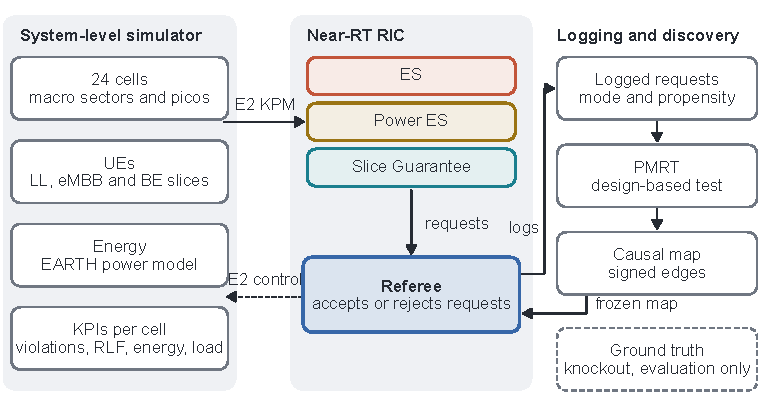
\includegraphics[width=\textwidth]{figures/fig_system.pdf}
\caption{System model.}
\label{fig:system}
\end{figure}

\subsection{Decision units and logging}
\label{sec:units}\claim{DEF-SYS-UNIT}\claim{DEF-SYS-LOG}

The referee decides per decision unit rather than per request. A unit $u$, identified by a cell, xApp and opening
time, opens at the pair's first request while none of its units is active. Its accept-or-reject mode $W_u$ is drawn
once and held for $t_{\mathrm{hold}} = 60$~s; all requests of the pair during the hold inherit it. The RIC records the
mode and its acceptance propensity $\pi_u$. Each unit also carries observation-only context from its opening request,
recent cell reports and applied configuration, including neighbour aggregates. Discovery uses only these logs and the
per-cell KPI series.

Three logging policies are considered. The uniform-randomised policy accepts each unit independently with probability
0.5. Under the state-dependent incumbent policy, the propensity, within $[0.15, 0.85]$, depends on the request class
and prior cell state: physical resource block (PRB) utilisation for energy-saving requests and the share of protected
user equipments (UEs) below their throughput floor for protected-share requests. Placebo logs draw and record modes
in the same way but apply every request.

\subsection{Problem formulation}
\label{sec:estimand}\claim{DEF-SYS-HYP}\claim{DEF-EST-H0}\claim{DEF-SYS-MITIG}

A hypothesis $(f, r, k)$ concerns a parameter family $f$, a relation $r$ and a KPI $k$; in the scenario of
Section~\ref{sec:design}, four families, three relations and five KPIs give $m = 60$ hypotheses. Because the referee
randomises the mode of a unit rather than a parameter value, each hypothesis concerns a mode contrast held for
$t_{\mathrm{hold}}$.
Let $y_u$ be the outcome of unit $u$ for $(r, k)$, namely the KPI summed over the cells of $r$ in the 90~s after
opening minus the same sum in the 90~s before. Let $\mathcal{F}_{u-1}$ denote the history of the network, of every
xApp and of the modes of earlier units up to the opening time. The xApp chooses the size of the change and the
direction $\mathrm{sgn}_u$ of the opening request, which orients the contrast, so that a positive effect means that
accepting a request that raises the parameter raises the KPI.

\begin{definition}[Policy-averaged assignment effect]
\label{def:tau_pi}\claim{DEF-EST-TAUPI}
Let $u$ be a unit of family $f$. Its assignment effect is
\begin{equation}
\tau_u^{\pi} = \mathbb{E}_{\pi}\bigl[y_u \mid \mathcal{F}_{u-1}, W_u = \text{accept}\bigr]
             - \mathbb{E}_{\pi}\bigl[y_u \mid \mathcal{F}_{u-1}, W_u = \text{reject}\bigr],
\label{eq:tau_u}
\end{equation}
where $\mathbb{E}_{\pi}$ averages over the network's future randomness and over the modes that the logging policy
$\pi$ draws for later units. The policy-averaged assignment effect $\tau_{\pi}$ of hypothesis $(f, r, k)$ is the
limit of $\bar\tau_{\pi} = N^{-1} \sum_u \mathrm{sgn}_u\, \tau_u^{\pi}$ over the $N$ units of $f$ as the number of
episodes grows.
\end{definition}

The target depends on the logging policy, which draws the modes of the other units in a unit's window, so randomised
and incumbent logs target different values of $\tau_{\pi}$. The knockout ground truth of Section~\ref{sec:gt} targets
a third contrast, $\tau_{\mathrm{AA}}$, in which every other unit is accepted. No
assumption of non-interference between cells or units is needed, because the null hypothesis concerns the whole
assignment vector of a family.

The paper addresses two problems. The first is discovery: from the logged units and KPI series alone, and without a
model of the network, test the sharp null $H_0(f, r, k)$ that the specified outcome is unchanged under every assignment
of $f$'s modes. Rejections form a signed causal effect map, with false discovery rate (FDR) control over these
sharp-null claims at a level $q$. The second
problem is mitigation: given such a map, choose a referee that minimises the protected-slice violations $V$ subject to
two safety constraints. First, the referee must keep at least 90~\% of the energy saving that the energy-saving xApps
achieve on their own. Second, each of four guard KPIs, namely the service violation rate, non-protected broadband
violations, low-latency violations and RLFs, must stay within 1.10 times its value under the static rule that accepts
every request (accept-all).

\section{Proposed framework}
\label{sec:method}

The framework has three components. The referee randomises its accept-or-reject decisions and
logs their propensities, which turns the controller's logs into an experiment with a known design. The predictable
matched-filter randomisation test (PMRT) uses this design to test each hypothesis of Section~\ref{sec:estimand} and
returns a signed causal effect map with asymptotic control of the FDR. A map-driven referee then uses the map to
reject harmful requests, and an edge-certification gate restricts it to rejections whose side effects on the guard
KPIs are certified small.

\subsection{Test statistic}
\label{sec:pmrt}\claim{DEF-PMRT-WEIGHT}

In reactive logs, network state drives both the mode $W$ and the KPIs. If the referee accepts when an independent
uniform draw $U$ falls below a logged propensity $\pi$, state affects the mode only through $\pi$. PMRT tests whether a
KPI moves with the modes more than those propensities predict, pairing a score of each mode with a weight built from
the KPI series and comparing the statistic with redraws from the logged design. It establishes whether an effect
exists, not its size.

Take a family $f$ and its units $u$ in information order: episode, opening time, cell. With $L(\text{accept}) = 1$ and
$L(\text{reject}) = 0$, the assignment score of unit $u$ is
\begin{equation}
v_u = \mathrm{sgn}_u \bigl( L(W_u) - \pi_u \bigr),
\label{eq:score}\claim{DEF-PMRT-SCORE}
\end{equation}
where $\mathrm{sgn}_u$ is the direction of the opening request. Over the policy's draw, $v_u$ has mean zero and
variance $\pi_u(1 - \pi_u)$, so an acceptance that was likely scores little and one against the odds scores more.
The weight $w_u$ summarises how the KPI under test moved after the unit opened. It is the residual of the KPI after a
ridge prediction~\cite{hoerl1970ridge} from what was known at opening, combined over the receiving cells and the
seconds after opening by a matched filter, then centred, shrunk and clipped~\cite{huber1964robust}. Every fitted part
was trained on earlier episodes, separate from the evaluation data (\esm{esm:method}).

The validity of the test rests on one property of the weight: apart from the KPI series under test, it uses only
information fixed before the unit drew its mode. It therefore uses no later unit, no unit of another family opening at
or after $u$, and no mean or slope over an episode's realised units, because whether those units exist can depend on
$W_u$. The statistic and its variance are
\begin{equation}
S = \sum_u v_u w_u, \qquad
\sigma^2 = \sum_u \pi_u (1 - \pi_u)\, w_u^2, \qquad
z = S / \sigma,
\label{eq:stat}\claim{DEF-PMRT-STAT}
\end{equation}
where $\sigma^2$ is the variance of $S$ over redraws of the modes with the weights held. Since it is the same for every
redraw, $z$ is normalised by the design variance rather than studentised. The reported sign is that of $S$ times an
orientation $o$, the sign of the training effect, which is set only when that effect is clear in the training data.

\subsection{Inference and false discovery rate control}
\label{sec:inference}\claim{DEF-PMRT-SUPPORT}\claim{DEF-FDR-WBY}\claim{ASM-A1-DESIGN}\claim{ASM-A2-NULL}\claim{ASM-A3-PRED}\claim{ASM-A4-REG}\claim{CIT-BY}\claim{CIT-RW}

The modes of family $f$ are redrawn $B$ times from the logged propensities, with every other family fixed and
the weights held, and $z_b$ is recomputed for each redraw. Each hypothesis has a two-sided p-value $p$ and, where $o$
is set, a one-sided value $p_d$ for each effect direction $d \in \{+1, -1\}$:
\begin{equation}
p = \frac{1 + \#\{b : |z_b| \ge |z|\}}{B + 1}, \qquad
p_d = \frac{1 + \#\{b : d\, o\, z_b \ge d\, o\, z\}}{B + 1},
\label{eq:pval}\claim{DEF-PMRT-PVAL}
\end{equation}
where $\#$ counts redraws. Algorithm~\ref{alg:pmrt} summarises the declaration pipeline; the complete per-hypothesis
algorithm and fixed support, window and weight-construction parameters are given in \esm{esm:method}. We use
$B = 9999$ redraws.

\begin{algorithm}[tbp]
\caption{PMRT declarations.}
\label{alg:pmrt}
\footnotesize
\begin{algorithmic}[1]
\Require hypotheses $\mathcal{H}$; training and evaluation units with modes, request directions, propensities and KPI
  series; redraws $B$
\Ensure signed declarations or untested hypotheses
\For{each hypothesis $j = (f, r, k) \in \mathcal{H}$}
  \State Check the required units, accepted and rejected modes, episodes and outcome windows; otherwise mark $j$
    untested
  \State On training episodes, fit the pre-window adjustment, matched filter, scale, clipping rule and prior direction
  \State For each evaluation unit in information order, compute its assignment score $v_u$ and outcome weight $w_u$
  \State Compute the observed statistic $z$ from Eq.~\eqref{eq:stat}
  \State Redraw the modes of family $f$ from their logged propensities $B$ times, holding the weights and other
    families fixed
  \State Compute the two-sided and available directional p-values from Eq.~\eqref{eq:pval}, with the reported sign
\EndFor
\State Apply the weighted BY step-up to all hypotheses; untested hypotheses are never declared
\State \Return the rejected hypotheses and their reported signs
\end{algorithmic}
\end{algorithm}

The sharp null $H_0(f, r, k)$ of Section~\ref{sec:estimand} is stated over possible units, because which units are
realised depends on the modes. The history $\mathcal{G}_{u-1}$ holds all other randomness and the modes of $f$'s first
$u - 1$ units, and the result rests on four assumptions.

\begin{description}
\item[(A1) Design.] For every unit $u$, its existence, cell, opening time, direction $\mathrm{sgn}_u$ and propensity
  $\pi_u$ are $\mathcal{G}_{u-1}$-measurable, $\Pr(W_u = \text{accept} \mid \mathcal{G}_{u-1}) = \pi_u$, and
  $\pi_{\min} \le \pi_u \le 1 - \pi_{\min}$ for a fixed $\pi_{\min} > 0$.
\item[(A2) Sharp null.] $H_0(f, r, k)$ holds.
\item[(A3) Predictable weights.] Every $w_u$ is $\mathcal{G}_{u-1}$-measurable and square integrable.
\item[(A4) Regularity.] As the number of episodes grows, the design variance $\sigma^2$ grows without any single unit
  dominating $S$.
\end{description}

Operationally, the RIC must draw each mode from its logged, past-determined propensity bounded away from 0 and 1; the
analyst must build each weight from information available when the unit opened, apart from the KPI under test; and the
log must contain enough units that none dominates $S$. In the simulator the last condition holds when clipping keeps
the weights bounded and $\sigma^2/n$ approaches a positive limit.

\begin{proposition}[Asymptotic validity of PMRT]
\label{prop:pmrt}\claim{ASM-ORIENT}\claim{THM-PMRT-ASY}
Assume (A1) to (A3). Then $S = \sum_u v_u w_u$ is a martingale with respect to $(\mathcal{G}_u)$, and its predictable
quadratic variation is $\sigma^2$. Let (A4) also hold and the number of episodes grow.
\begin{enumerate}
\item The statistic $z = S / \sigma$ converges in distribution to $\mathcal{N}(0, 1)$.
\item Conditionally on the data, every redraw $z_b$ has mean 0 and, where $\sigma > 0$, variance 1, and its distribution
  function converges uniformly to $\Phi$ in probability.
\item For every fixed $B$ and every $t \in [0, 1]$, $\limsup \Pr(p \le t) \le \lfloor t(B + 1) \rfloor / (B + 1) \le t$.
  The same holds for $p_d$ for each $d$ when $o$ is fixed in advance.
\end{enumerate}
The p-values $p$ and $p_d$ are therefore asymptotically valid. The value $p$ differs from
$2\{1 - \Phi(|z|)\}$ only by a term that vanishes in probability and by Monte Carlo error.
\end{proposition}

Adaptive unit creation, repeated requests and state-dependent propensities do not invalidate the martingale argument
when their existence, timing and propensity are determined before the current mode is drawn, as (A1) requires. The
fresh-draw lemma\claim{THM-FRESH} (\esm{lem:s_fresh}) then gives each assignment score conditional mean zero, so under
the sharp null $S$ has predictable variance $\sigma^2$ in every sample. Assumption (A4) supplies the asymptotic
calibration through the martingale central limit theorem~\cite[Cor.~3.1 and 3.2]{hall1980martingale}\claim{CIT-HH} and
the Lindeberg--Feller and P\'olya theorems~\cite[Thm.~3.4.10 and Exercise~3.2.9]{durrett2019probability}\claim{CIT-DUR}.
The redraw p-value is nevertheless not exact in finite samples: changing a mode can alter the later network state,
units and propensities, so the adaptive design cannot generally be replayed as required by exact sequential
randomisation tests~\cite{bojinov2019timeseries}. A fixed design gives a valid tie-inclusive p-value\claim{THM-EXACT},
exact for a continuous statistic~\cite[Sect.~4]{phipson2010permutation}\claim{CIT-PS}, but PMRT does not meet that
condition; a two-unit counterexample is given in \esm{ex:s_adaptive}\claim{THM-COUNTEREX}. The placebo and null-outcome
experiments of Section~\ref{sec:res_validity} assess finite-sample behaviour.

The 60 hypotheses are declared together by a weighted Benjamini--Yekutieli (BY)
step-up~\cite[Thm.~1.3]{benjamini2001dependency}, \cite{blanchard2008fdr} at $q = 0.05$. Hypothesis $j$ enters with
training-derived weight $\omega_j$ and, when available, prior-direction p-value $p_{d_j}$; otherwise it enters with
$p$~\cite[Thm.~3.1 and Sect.~5]{roeder2009weighted}. A rejection is reported with that prior direction or the test's
reported sign.

\begin{corollary}[Asymptotic false discovery rate]
\label{cor:fdr}\claim{ASM-FDR-FIXED}\claim{THM-FDR-ASY}
Let $\mathcal{H}_0$ hold the true sharp nulls among the $m = 60$ hypotheses. Let (A1) to (A4) hold for each of them,
and let the weighted step-up use directions $d_j$ and weights $\omega_{n,j} \ge 0$ with $\sum_j \omega_{n,j} = m$ for
the analysed sample size $n$, all fixed from data independent of the evaluation data, with $\omega_{n,j} \to \omega_j$
(or $\omega_{n,j} = \omega_j$ for every $n$). Then, whatever the dependence between the p-values,
\begin{equation}
\limsup_{n \to \infty} \mathrm{FDR} \le \frac{q}{m} \sum_{j \in \mathcal{H}_0} \omega_j \le q,
\label{eq:fdr}
\end{equation}
where a false discovery is the rejection of a true sharp null.
\end{corollary}

The result applies the reshaped weighted step-up of Blanchard and Roquain~\cite[Thm.~4.2]{blanchard2008fdr}
\claim{CIT-BR} through a finite-sample bound with asymptotically vanishing slack\claim{THM-BY-FIN}
(\esm{esm:theory}). Counting untested hypotheses in $m$ is conservative because they are never declared.

\subsection{Scope of the guarantees}
\label{sec:reading}\claim{THM-SCOPE}

A declared edge states that the modes of family $f$ change KPI $k$ somewhere in the cells that relation $r$ covers,
and the FDR bound covers that claim asymptotically. It does not cover the reported sign, effect magnitude or unique
spatial attribution: a unit's neighbour and far cells are the own cells of other units of $f$, so an effect of $f$ on
its own cells also moves the KPI of their neighbour and far cells, and the far hypotheses are no negative control
(\esm{tab:s_attr}). Table~\ref{tab:terms} summarises these distinctions. The gate similarly screens undeclared guard
edges but does not certify the resulting policy, whose constraints are evaluated on held-out seeds.

\subsection{Map-driven referee}
\label{sec:slope}\claim{ASM-SLOPE-CENTRE}
\label{sec:referee}\claim{DEF-REF-RULES}

The referee needs the size of each effect, not only its sign, and takes it from the design slope $\hat\beta$, which
regresses each unit's centred outcome on its assignment score. Let $e_u = y_u - \tilde y_u$ be the outcome minus an
outcome centre $\tilde y_u$ computed from earlier units' outcomes and $u$'s pre-window. Under the uniform-randomised policy,
\begin{equation}
\hat\beta = \frac{\sum_u v_u e_u}{\sum_u v_u^2}
          = \frac{1}{N} \sum_u \mathrm{sgn}_u \Bigl( \frac{\mathbf{1}\{W_u = \text{accept}\}\, e_u}{\pi_u}
            - \frac{\mathbf{1}\{W_u = \text{reject}\}\, e_u}{1 - \pi_u} \Bigr),
\label{eq:slope_ht}\claim{DEF-SLOPE}
\end{equation}
with $\pi_u = 0.5$, which is the Horvitz--Thompson estimator of $\tau_{\pi}$ and converges to it
(design-slope lemma, \claim{THM-SLOPE}\esm{esm:theory}). Under a state-dependent policy such as the incumbent, it converges to the
$\pi_u(1 - \pi_u)$-weighted average of $\mathrm{sgn}_u \tau_u^{\pi}$. The lemma assumes an outcome centre fixed before
$u$'s mode is drawn, which the implemented centre meets only approximately (Section~\ref{sec:disc_limits}).

A causal effect map $M$ gives each declared edge $(f, r, k)$ a signed coefficient $\beta(f, r, k)$. For PMRT it is the
declaration's sign times the magnitude of the design slope; an associational map uses the method's sign times the
magnitude of the least-squares slope of the outcome on the logged mode. The referee decides when a decision unit opens,
on the opening request's family, direction and context, and later requests of the pair inherit the mode. For a request
of family $f$ and direction $d$ it sums the direction-adjusted effects $\Delta_k = d \sum_r \beta(f, r, k)$ over the
own, neighbour and far relations for each KPI $k$, judges the request on the first KPI with $\Delta_k \ne 0$ in the
order protected-slice violations, service violations, RLFs, and rejects it if it is harmful and either costly in energy
or under protected-UE pressure. A rejection that accepting would have helped on a guard KPI is delayed by at most one
unit. The same constants apply to every map; the full rules are in \esm{esm:method}.

\subsection{Edge-certification gate}
\label{sec:gate}\claim{DEF-GATE}\claim{ASM-GATE-COV}\claim{THM-GATE-BUDGET}

A map leaves some guard edges undeclared, and a referee acting on it can harm a guard KPI through such an edge. The
gate prevents this by letting the referee reject a class of requests only when every undeclared guard edge of the
class is certified small. It checks every class $(f, d)$ that the referee can reject against the own, neighbour and far
relations of the two guard KPIs, service violations and RLFs. Rejecting a request of direction $d$ moves a guard KPI
by $-d\,\beta$, so a rejection's harmful direction is $h = -d$. We write the class $(f, +1)$ of requests that raise $f$
as $f$-up, so that sleep-up holds the requests to put a pico to sleep, and $(f, -1)$ as $f$-down.

An undeclared edge is certified when the one-sided 90~\% upper bound of $h\,\beta$ from the map's own estimator is at
most a tolerance $\varepsilon(f, d, k)$, and is otherwise unresolved; a class with any unresolved edge is always
accepted, and a map without an effect estimator cannot certify. The tolerance is
\begin{equation}
\varepsilon(f, d, k) = \frac{0.05\, G_k}{3\, \max\{N(f, d), 1\}},
\label{eq:tol}
\end{equation}
with $G_k$ the mean per-episode total of guard KPI $k$ and $N(f, d)$ the mean number of units of the class per
episode, both measured under accept-all on development episodes. Suppose that every unit of a class were rejected,
that the class had at most $\max\{N(f, d), 1\}$ units, and that each rejection moved the KPI by at most $\varepsilon$ on
each of the three relations. The guard ratio would then move by at most 0.05, half the margin of 0.10 that a referee
may use under the 1.10 limit of Section~\ref{sec:estimand}. The certificate is thus a first-order budget per edge, not
a bound on the referee's guard ratios: it ignores overlapping windows, classes acting together and declared edges, so
whether a referee meets its guards is checked on held-out seeds.

\section{Experimental setup}
\label{sec:design}

We evaluate discovery and closed-loop mitigation in a system-level O-RAN surge simulation, and isolate the role of
the logging design in controlled environments with known causal structure.

\subsection{Simulation environment and scenario}
\label{sec:scenario}\claim{DEF-SIM-CONST}

The simulator models a near-RT RIC and the RAN it controls (Figure~\ref{fig:system}). The network has 24 cells: 21
macro sectors on a seven-site hexagonal layout~\cite{3gpp36814} and three co-channel picos at traffic hotspots, serving
300 UEs in a low-latency (LL), an enhanced mobile broadband (eMBB) or a best-effort slice. Traffic, mobility and a
hidden per-site load process come from an exogenous tape keyed by the seed, so that runs that act differently see the
same tape (parameters in \esm{esm:setup}). In the surge scenario, a localised surge triples the file-arrival rate of the UEs
near a venue during the middle of the scored window.

Three xApps run on the RIC, each writing its own parameter families (Table~\ref{tab:xapps}). The Energy Saving (ES)
xApp switches macro carriers and puts picos to sleep using the load-time thresholds of 3GPP TS 28.541~\cite{3gpp28541},
and the Power ES xApp backs off the macro transmit power as in 3GPP TR 38.864~\cite{3gpp38864}. The Slice Guarantee
xApp sets the protected minimum PRB share that serves a protected subset of the eMBB UEs. The result is a three-way
indirect conflict without a shared parameter: the energy-saving xApps act on the KPIs of neighbouring cells, and Slice
Guarantee on the protected-slice violations of its own cell. The edge from pico sleep to neighbour protected-slice
violations is the one on which the conflict rests: since the protected share moves only its own cell's protected-slice
violations, a referee that rejects Slice Guarantee's requests removes the protection that the energy-saving xApps
erode.

\begin{table}[tbp]
\caption{xApps of the surge scenario.}
\label{tab:xapps}
\setlength{\tabcolsep}{4pt}
\begin{tabular}{@{}p{2.2cm} p{3.5cm} p{3.0cm} p{3.5cm}@{}}
\toprule
xApp & Parameter & Range & Acts when \tabularnewline
\midrule
\raggedright ES & \raggedright Macro carrier; pico sleep & \raggedright on/off; awake/asleep & \raggedright load low / high \tabularnewline
\raggedright Power ES & \raggedright Macro transmit-power offset & \raggedright $-9$ to 0~dB & \raggedright load low / high \tabularnewline
\raggedright Slice Guarantee & \raggedright Protected minimum PRB share & \raggedright 0 to 0.5 & \raggedright protected UEs below floor \tabularnewline
\bottomrule
\end{tabular}
\end{table}

\subsection{Datasets}
\label{sec:datasets}\claim{PRO-TUNE}

Discovery uses uniform-randomised and state-dependent logs of 600 evaluation episodes each, matched placebo logs, and
null outcomes formed by cyclically shifting KPI series across episodes. Unlike placebos, the null outcomes retain the
re-proposals and state-dependent propensities. Maps learned from the state-dependent logs drive ungated and gated
referees on separate fresh seeds; the gate is calibrated on \val{s3.gate.dev_episodes} development episodes. All
methods and baseline thresholds are tuned on development episodes separate from evaluation.

\subsection{Knockout ground truth}
\label{sec:gt}\claim{DEF-GT-LABEL}

The maps are scored against knockout rollouts, which estimate the effect of one unit's mode with every other unit
accepted; as this target is not PMRT's $\tau_{\pi}$, the scores measure agreement rather than the validity of the
test.

\begin{definition}[Knockout effect]
\label{def:tau_aa}\claim{DEF-EST-TAUAA}
Let $u$ be a unit sampled on separate episodes. Its knockout effect $\tau_u^{\mathrm{AA}}$ is the accept-minus-reject
difference of the KPI summed over the cells of $r$ in the 90~s after opening, in rollouts from the copied state with
every other unit accepted. The knockout effect $\tau_{\mathrm{AA}}$ is the mean of $\mathrm{sgn}_u\,
\tau_u^{\mathrm{AA}}$ over the sampled units.
\end{definition}

Pooling the units of a family over \val{s1.gt.episodes} ground-truth episodes gives a mean per hypothesis with a 95~\%
episode-cluster bootstrap interval. A hypothesis is labelled true, with the sign of its mean, when the interval
excludes zero and the absolute mean is at least a materiality threshold $\delta_k$, set to 5~\% of the largest
absolute mean of KPI $k$. It is labelled knockout-null when the interval lies within $\pm\delta_k$, and is otherwise
left unscored. This is a practical-equivalence label rather than PMRT's sharp null (Table~\ref{tab:terms}), and it
depends materially on $\delta_k$ (\esm{esm:discovery}). On the uniform-randomised logs the ground truth labels 29 of the 60 hypotheses true, 21 null and 10
indeterminate (\esm{esm:setup}).\claim{EMP-GT-LABELS}

\subsection{Controlled environments}
\label{sec:envs}\claim{DEF-ENV}\claim{DEF-ENV-ARMS}\claim{ASM-S4-KNOWN}

The simulator runs one scenario with one logging design per dataset, and its ground truth is estimated. The controlled
environments remove both limitations: each isolates one mechanism with a known causal graph, so that every null edge
is null by construction, and the same mechanism is logged under several designs. The five environments contain a
clean linear graph, an edge active only in a rare regime, delayed harm through lagged KPI cascades, latent
confounding, and the three mechanisms composed (Figure~\ref{fig:envs}a). Actions are logged by independent redraws per
observation, by a dithered setpoint held for a twentieth of the data plus a small independent dither, or, in the
latent-confounding environment, by a confounded behaviour policy with logged probabilities (Figure~\ref{fig:envs}b).
Each method ran at 500 to 24\,000 observations, and each condition on 40 seeds. A null-edge rate is invalid when the
lower bound of its 95~\% seed-cluster bootstrap interval exceeds 0.05, valid when the upper bound is at most 0.075, and
inconclusive otherwise; a condition is invalid when any of its rates is.

\begin{figure}[tbp]
\centering
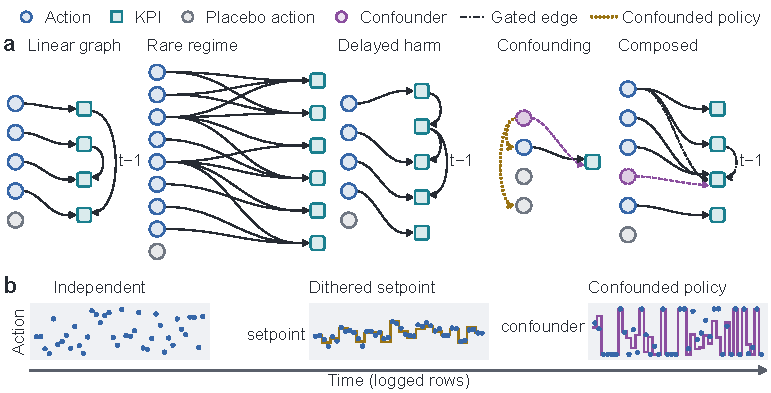
\includegraphics[width=\textwidth]{figures/fig_envs.pdf}
\caption{Controlled environments and logging designs.}
\label{fig:envs}
\end{figure}

Three groups of tests are compared. Design-based tests redraw the logged design: PMRT-GBM, which uses a
gradient-boosting statistic and plain BY control at $q = 0.05$, and its linear counterpart PMRT-Lin.
Design-adjusted tests condition on the logged design variables: partial correlation, Granger and
RCoT~\cite{strobl2019rcot}. Design-blind methods ignore those variables: correlation; partial correlation
with standard or heteroskedasticity- and autocorrelation-consistent errors~\cite{newey1987hac,kiefer2005fixedb};
Granger; RCoT; PC~\cite{spirtes2000causation}; NOTEARS~\cite{zheng2018notears}; SHAP-DAG after Sharma et
al.~\cite{Sharma_2025,lundberg2017shap}; the two-tower network; our earlier max-stratified
correlation-ratio test; and CDD O-RAN's discovery stage~\cite{dahal2026cddoran}. These environments isolate
the randomisation construction shared by the PMRT variants, not the simulator PMRT's matched-filter
statistic or weighted declaration layer; its validity therefore rests on the simulator null checks in
Section~\ref{sec:res_validity}.

\subsection{Baselines and metrics}
\label{sec:baselines_scores}\claim{DEF-MET-MAP}\claim{DEF-MET-DEC}

In the simulator, PMRT is compared with seven associational baselines that ignore the logging design and run on the
same unit table (\esm{esm:setup}): correlation, Granger~\cite{granger1969causal} with a tuned threshold or under BY control
(Granger~+~BY), SHAP-GBDT~\cite{Sharma_2025}, a two-tower network~\cite{santos2026conflictairan}, the intent-conflict
statistic INT of PACIFISTA~\cite{PACIFISTA} and QACM~\cite{QACM2024}. Each threshold was set on development episodes so
that the far relation received at most one declaration. Because the ground truth labels \val{s1.far.true} of the
\val{s1.far.total} far hypotheses true on the uniform-randomised logs and \val{s2.far.true} on the state-dependent logs, this rule
caps the recall a baseline can reach. On the uniform-randomised logs the baselines' placebo declarations come from their
thresholds rather than from confounding, and on the state-dependent logs the baselines are also reported at thresholds
calibrated on placebo logs.

Maps are scored over the \val{s1.gt.hypotheses} hypotheses; indeterminate labels count in neither precision nor
recall, F1 is their harmonic mean, and sign accuracy is the share of declared true edges with the ground-truth sign.
Referees are compared with accept-all, never-sleep, single-xApp subsets, and referees driven by the oracle, random and
associational maps (\esm{esm:setup}). Protected-slice violations $V$ define the recovery
$R = (V_{\mathrm{AA}} - V)/(V_{\mathrm{AA}} - V_{\mathrm{ref}})$, which is 0 for accept-all and 1 for the best
single-xApp subset. Eligibility requires the constraints of Section~\ref{sec:estimand}; never-sleep is the best
eligible static rule because the subset attaining $R = 1$ retains almost no energy saving. Decision intervals are
90~\% paired seed-bootstrap intervals and rate intervals are 95~\% cluster-bootstrap intervals.

% Step 5 rewrite (2026-10-14): Results. Merges old Section 6 (discovery), the results of old Section 7 (controlled
% environments) and old Section 9 (decisions), ordered by RQ1-RQ3. New figures (Step 3, user-approved): fig_placebo,
% fig_maps, fig_logging_validity, fig_decisions; they replace fig_study1_discovery, fig_study2_maps,
% fig_study4_validity and fig_decision_referee. Moved to Appendix D: the validity table, the full map table with the
% placebo-calibrated and existence panels, the controlled-environment claims table, the full decision scorecard and the
% gate diagnosis. Every number is copied from the old sections and tables (journal ec32c22) or the figure modules'
% build-time assertions; the confounded-policy design-blind rates are from
% reviews/2026-10-13/briefs/N3_confounded_designblind.md (report.json V1_validity + V6_E4).
\section{Results}
\label{sec:results}

This section reports the results in the order of the research questions: the validity of the test
(Section~\ref{sec:res_validity}), the agreement with the ground truth (Section~\ref{sec:res_map}), the
role of the logging design in the controlled environments (Section~\ref{sec:study4}), and the conflict-mitigation
decisions (Section~\ref{sec:res_decision}).

\subsection{Validity}
\label{sec:res_validity}

PMRT made no declaration on the placebo logs of either dataset or on the null outcomes, and it met every validity
check of the protocol (Appendix~\ref{app:validity}). The baselines, in contrast, declared edges on placebo logs, up to
13 on the randomised logs and up to 29 on the confounded logs (Figure~\ref{fig:placebo}). Because the modes of the
randomised logs are independent of the network state, the declarations there arise from the baselines' thresholds
rather than from confounding. On the confounded logs, four of the seven baselines declared more placebo edges than on
the randomised logs, which is consistent with confounding adding to the threshold effect.

\begin{figure}[tbp]
\centering
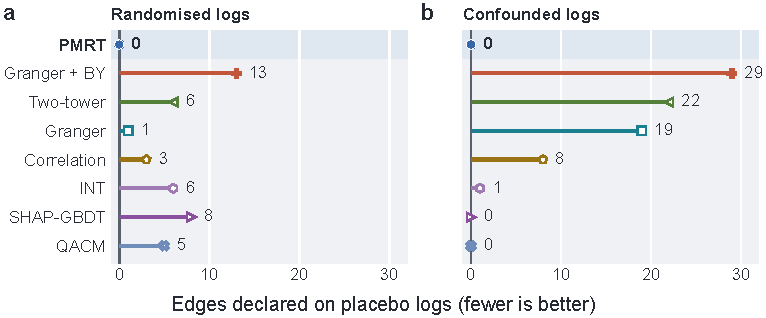
\includegraphics[width=\textwidth]{figures/fig_placebo.pdf}
\caption{Edges declared on placebo logs.}
\label{fig:placebo}
\end{figure}

The validity checks also showed three departures from exactly nominal behaviour, none of which led to a declaration.
On the randomised placebo logs, 7 of the 60 p-values were at or below 0.05 where 3 were expected; the binomial tail
probability of 0.03 remained above the protocol limit of 0.01. The null-outcome check used 999 redraws, with which a
declaration was unattainable, so it was repeated with 9\,999 redraws, which produced declarations in 2 of 590
variants, within the limit of 7.5~\%. Finally, the hypotheses that the ground truth labels
null are small effects rather than sharp nulls. Over all 21, the rate of p-values at or below 0.05 was 0.15, about
three times nominal, which reflects real effects below the materiality threshold. Over the 12 whose knockout interval
also contains zero it was 0.075, with an interval reaching 0.16, so that an excess cannot be excluded there either.

\subsection{Agreement with the ground truth}
\label{sec:res_map}
\label{sec:study1}
\label{sec:study2}
\label{sec:map_claims}

PMRT's maps agreed closely with the knockout ground truth (Figure~\ref{fig:maps}). On the randomised logs it declared 28
edges, with a precision of 0.92, a recall of 0.79 and no wrong sign. On the confounded logs, where the incumbent's
state-dependent propensities were logged, it declared 22 edges, with a precision of 0.86, a recall of 0.62 and again no
wrong sign (Table~\ref{tab:maps}). It declared the edge from pico sleep to neighbour protected-slice violations, on which the
scenario's conflict rests, and the other three edges of the conflict chain, each with the ground-truth sign, on both
kinds of log and in every larger subsample of the randomised logs. Of the ten true neighbour-relation edges it declared nine,
missing only the edge from pico sleep to neighbour RLFs. The baselines either declared far fewer true edges or reached
a higher recall only with wrong signs and false edges. Granger~+~BY, the strongest of them, reached a recall of 0.55 with six
wrong signs on each kind of log and a precision of 0.59 and 0.54. Calibrating the baselines' thresholds on the placebo
logs themselves removed their placebo declarations, but only in-sample and at the cost of recall, which fell to at
most 0.21 (Appendix~\ref{app:maps_full}).

\begin{figure}[tbp]
\centering
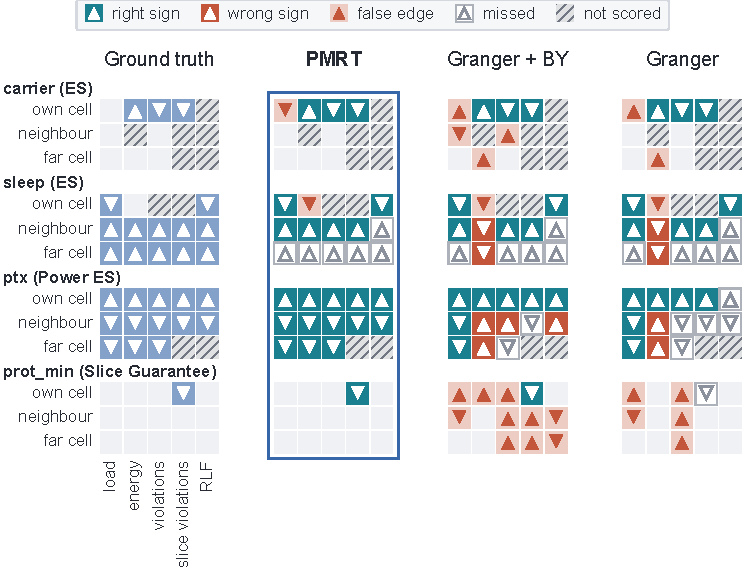
\includegraphics[width=\textwidth]{figures/fig_maps.pdf}
\caption{Causal maps learned from randomised logs.}
\label{fig:maps}
\end{figure}

\begin{table}[tbp]
\caption{Map quality on randomised / confounded logs.}
\label{tab:maps}
% Precision = (R + W) / (R + W + N) and recall = right-sign recall over the 29 true hypotheses, from the old
% tab:maps (journal ec32c22), DEV-tuned thresholds; placebo edges as in fig_placebo.
\setlength{\tabcolsep}{4pt}
\begin{tabular*}{\textwidth}{@{\extracolsep{\fill}}l c c c c@{}}
\toprule
Method & Precision & Recall & Wrong signs & Placebo edges \\
\midrule
PMRT         & 0.92 / 0.86 & 0.79 / 0.62 & 0 / 0 & 0 / 0 \\
Granger + BY & 0.59 / 0.54 & 0.55 / 0.55 & 6 / 6 & 13 / 29 \\
Granger      & 0.69 / 0.60 & 0.48 / 0.41 & 4 / 6 & 1 / 19 \\
QACM         & 0.89 / 0.83 & 0.28 / 0.17 & 0 / 0 & 5 / 0 \\
INT          & 0.88 / 0.80 & 0.24 / 0.14 & 0 / 0 & 6 / 1 \\
Correlation  & 0.86 / 0.80 & 0.17 / 0.21 & 1 / 2 & 3 / 8 \\
Two-tower    & 1.00 / 0.63 & 0.17 / 0.17 & 1 / 0 & 6 / 22 \\
SHAP-GBDT    & 1.00 / 0.50 & 0.03 / 0.03 & 0 / 0 & 2 / 2 \\
\bottomrule
\end{tabular*}
\end{table}

One protocol criterion on the randomised logs was not met. It required PMRT's F1 score on the neighbour-relation edges
to equal or exceed that of each of three baselines on most small subsamples. Against Granger~+~BY the condition held on only 2
of the 10 smallest subsamples, although it held on 4 of the 5 larger ones, so that the discovery verdict on these logs
was partial (Online Resource~1, Section~S1.1). The F1 ranges of the two methods overlapped on the smallest subsamples, and
the criterion did not account for the 13 placebo edges of Granger~+~BY. Discovery on the confounded logs met every
criterion.

Precision depends on how the ground truth is defined. Against the materiality threshold used throughout, it was 0.92
and 0.86;
with the threshold halved it rose to 1.00 on both kinds of log, and with it doubled it fell to 0.59 and 0.73. The fall
reflects real effects below the doubled threshold rather than wrong declarations. Under an existence rule, which
counts any effect whose knockout interval excludes zero, 26 of PMRT's 28 declarations on the randomised logs and all
22 on the confounded logs were real effects with the declared sign (Appendix~\ref{app:x11}). PMRT made no wrong-sign
declaration under any ground-truth variant, and its neighbour and far declarations were almost all labelled true, 12 of
13 on the randomised logs and all 7 on the confounded logs. Under the doubled threshold, however, the ranking of
methods is not preserved: the small maps of INT, QACM and two-tower kept precisions of 0.88, 0.80 and 0.83 on the
randomised logs, above PMRT's 0.59, although at recalls of 0.35, 0.40 and 0.25 against its 0.80.

\subsection{Role of the logging design}
\label{sec:study4}
\label{sec:study4_results}
\label{sec:study4_verdicts}

The controlled environments confirm that validity derives from the logging design. Tests that ignored the design
were close to their nominal rate under independent logging but lost it once actions followed a dithered setpoint, with
null-edge rates of 0.33 to 0.94, whereas the design-based and design-adjusted tests remained near 0.05 under every
logging design (Figure~\ref{fig:logging_validity}). All four claims fixed in the protocol were supported
(Online Resource~1, Section~S4.1), with two exceptions. Design-adjusted RCoT was invalid even with the design covariates,
and PMRT-Lin, the secondary linear variant, exceeded its allowance of invalid conditions under the confounded policy,
although its pooled rates were valid and a re-run on fresh datasets gave rates consistent with chance.

\begin{figure}[tbp]
\centering
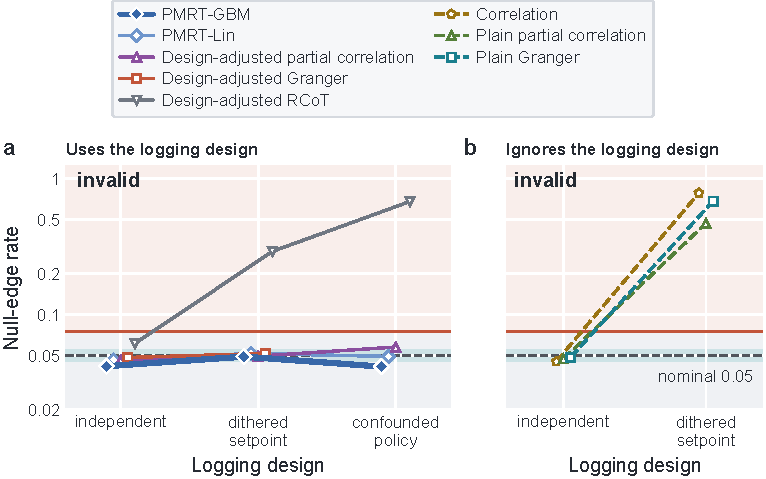
\includegraphics[width=\textwidth]{figures/fig_logging_validity.pdf}
\caption{Null-edge rate by logging design.}
\label{fig:logging_validity}
\end{figure}

The latent-confounding environment illustrates the mechanism most directly, because there the associational sign is
reversed at large confounding strength. Under the logged confounded policy, the null-edge rate of correlation was 1.00 whenever the
confounding was present, while that of PMRT-GBM stayed between 0.02 and 0.06 in every condition. Validity under this
policy is not specific to PMRT: design-adjusted partial correlation also stayed valid. The protocol did not score the
design-blind tests under the confounded policy; descriptively, correlation and plain RCoT were far above nominal there,
at 0.77 and 0.23, whereas plain partial correlation stayed near nominal, at 0.056, most likely because the confounder
was among its covariates. A post hoc variation of the dither width and of the number of setpoints left correlation
invalid and the two PMRT methods between 0.042 and 0.054. Under unlogged confounding, the negative control, the real
actions have no logged design, and on the placebo edge the rates of the design-based tests were never invalid.

The same environments also show the limits of a placebo check. With its threshold calibrated on the placebo column,
the discovery stage of CDD O-RAN passed that check but exceeded the nominal null-edge rate in 9 of 30 conditions. A
pipeline that declares placebo edges, as every baseline did on the randomised logs, is thus shown to be invalid, whereas
a pipeline that passes the check may still be invalid. The check is therefore a necessary condition for validity, but
not a sufficient one.

\subsection{Conflict mitigation}
\label{sec:res_decision}
\label{sec:res_referee}
\label{sec:study3}

Without the gate, the PMRT referee reached the highest recovery of any referee, $R = 0.47$, but breached the RLF guard
and was therefore ineligible (Figure~\ref{fig:decisions}, Table~\ref{tab:decision_e2e}). Its RLF ratio was 1.31
(90~\% confidence interval, CI, 1.10 to 1.56), against the limit of 1.10. The breach came from rejected transmit-power requests.
PMRT's map from the confounded logs lacked the edge from the transmit-power offset to neighbour RLFs, which the ground
truth labels true; the oracle map holds this edge, so its guard-conflict rule accepts the next power-up unit after each
rejected one. Over all seeds, PMRT's referee rejected 8\,674 power-up units against the oracle map's 2\,370, while
their sleep rejections were similar. PMRT's primary statistic had missed this edge ($p = 0.49$); an unfiltered
statistic, examined after the fact and not used, would have detected it.

\begin{figure}[tbp]
\centering
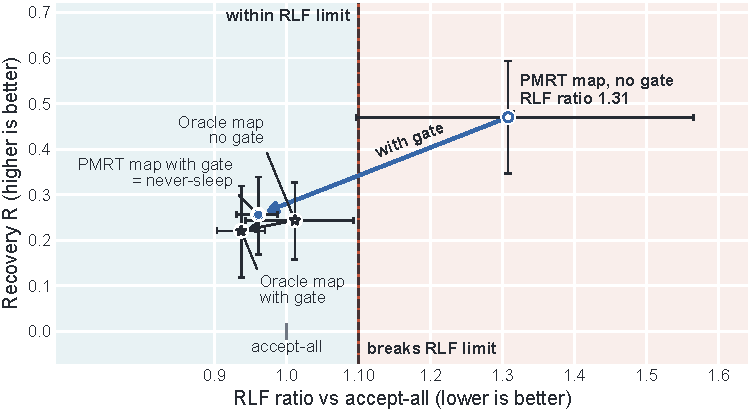
\includegraphics[width=\textwidth]{figures/fig_decisions.pdf}
\caption{Recovery against RLF ratio, without and with the gate.}
\label{fig:decisions}
\end{figure}

\begin{table}[tbp]
\caption{Decision outcomes.}
\label{tab:decision_e2e}
% From the old full scorecard (now Table tab:decision_full in Appendix D); 90 % paired seed-bootstrap CIs.
\setlength{\tabcolsep}{4pt}
\begin{tabular*}{\textwidth}{@{\extracolsep{\fill}}l c c c c@{}}
\toprule
Arm & $R$ & $R$ minus never-sleep [90~\% CI] & RLF ratio & Eligible \\
\midrule
\multicolumn{5}{@{}l}{\textit{Without the gate}} \\
\quad Accept-all & 0.00 & $-0.22$ [$-0.30$, $-0.14$] & 1.00 & yes \\
\quad Never-sleep & 0.22 & -- & 0.99 & yes \\
\quad PMRT map & 0.47 & $+0.25$ [$0.14$, $0.36$] & 1.31 & no \\
\quad Oracle map & 0.24 & $+0.02$ [$-0.04$, $0.09$] & 1.01 & yes \\
\midrule
\multicolumn{5}{@{}l}{\textit{With the gate}} \\
\quad Accept-all & 0.00 & $-0.26$ [$-0.34$, $-0.17$] & 1.00 & yes \\
\quad Never-sleep & 0.26 & -- & 0.96 & yes \\
\quad PMRT map & 0.26 & $0.00$ [$0.00$, $0.00$] & 0.96 & yes \\
\quad Oracle map & 0.22 & $-0.04$ [$-0.10$, $0.03$] & 0.94 & yes \\
\bottomrule
\end{tabular*}
\end{table}

With the gate, the PMRT referee met every guard but made the same decisions as the never-sleep rule: on every seed its
outcomes were identical to those of never-sleep, so its gain in recovery over that rule, the primary criterion, was
zero. The protocol had anticipated this tie and kept the criterion unchanged, since dropping it would have changed a
criterion in view of an expected result. No gated referee improved on never-sleep; the oracle map differed from it by $-0.04$ (90~\% CI $-0.10$ to
$0.03$). The gated runs used fresh seeds, and on them the ungated PMRT referee, run as a descriptive arm, no longer
outperformed never-sleep, differing by $-0.06$ at an RLF ratio of 1.05. Pooled over both seed sets, its gain was small, 0.10 with an
interval that barely excludes zero, and its RLF ratio of 1.18 still breached the guard. The two seed sets did not
differ at the network level, but the referee's per-seed gain was heavy-tailed and its mean differed between them. The
rule stated in advance did not cover this case, so the non-replication was attributed after the results had been seen
to seed-level heterogeneity of an adaptive referee, and the pooled estimate is taken as the best estimate
(Appendix~\ref{app:x15}).
Referees using the associational maps, finally, raised protected-slice violations to 4.5 to 5.4 times the accept-all
level, because they rejected Slice Guarantee's protected-share requests; several stayed eligible, since the protected
slice has no guard of its own (Appendix~\ref{app:decision_full}).

\label{sec:disc_decision}
The gate accounts for the absence of a gain from a valid map. Of the request classes that the PMRT map allows the
referee to reject, the gate certified only putting picos to sleep. It withheld the transmit-power-up rejections because their two
unresolved guard edges, to neighbour RLFs and far service violations, are true in the ground truth, with point
estimates of harm above their tolerances, so that more logging would not have certified them (Appendix~\ref{app:gate}).
The oracle map certifies this class only because it declares both edges, and its gated referee gained over never-sleep
only in energy retention, 1.29 against 1.15. Rejecting more requests does not compensate for this: a referee that rejected
requests at random, at the rate of the ungated referee, had negative recovery. In this scenario, therefore, the guards
and the objective, rather than the map, limited the benefit of safe decisions.

\section{Discussion}
\label{sec:discussion}

The results support two findings of different strength. The validity of a test that uses the logged design follows from
its construction and was confirmed on placebo logs, on null outcomes and in controlled environments with known causal
graphs. The finding that a valid map did not improve safe conflict mitigation, in contrast, rests on a single simulated
scenario and a single referee rule.

\subsection{Implications for causal discovery}
\label{sec:disc_discovery}\claim{EMP-POWER}

The validity of the test derives from the logged design rather than from a model of the network, which makes it the
property most likely to transfer to other networks. The randomisation distribution is generated from the logged
propensities alone, whether uniform or state-dependent, so the guarantee holds for any statistic, weighting or prior
direction fixed before each unit draws its mode. The controlled environments confirm that this guarantee belongs to the
design rather than to PMRT, since partial correlation adjusted for the design variables also retained its nominal rate
under a logged state-dependent policy.

Statistical power, in contrast, depends on the choice of statistic. Design-adjusted partial correlation had higher recall in the
latent-confounding environment, whereas PMRT had higher recall on the uniform-randomised simulator logs. PMRT's
matched filter and weights therefore concern power rather than the source of validity.

\subsection{Implications for conflict mitigation}
\label{sec:disc_mitigation}

In the evaluated scenario, mitigation was limited by the guard constraints and objective, not by map accuracy. With
the gate, the PMRT referee made the same decisions as the never-sleep rule, and the oracle map performed no better.
Further improvements in discovery would therefore not have increased the benefit of safe mitigation here. Conversely,
the ungated result shows that one missed edge was sufficient for the referee to breach a guard limit. A map should therefore not drive
mitigation without a step that certifies the effect of each decision on every guard KPI.

\subsection{Deployment requirements}
\label{sec:disc_deploy}\claim{EMP-X3}\claim{EMP-S1-STRICT}\claim{EMP-X4}

The test requires the conflict-mitigation layer to draw each accept-or-reject decision with a known propensity and
record it exactly. The policy may change over time, provided that each recorded propensity is the one used for the
draw. Otherwise the design is misspecified: in the controlled environments, PMRT-GBM and PMRT-Lin exceeded the
nominal null-edge rate when the assumed dither width was 0.8 times the true width, and every PMRT variant did so when
the assumed logging-policy strength was twice its true value (\esm{esm:envs}). The RIC should therefore record the
propensity at the moment of the draw, from the code that performs it, and keep propensities bounded away from 0 and 1.

Randomised logging imposes policy and evidence costs. Random rejection reduced recovery below accept-all because it
rejected requests that a fixed rule would accept. Evidence also accumulates at the rate of decision units, each a 60~s
mode followed by a 90~s outcome window, rather than at the RIC control-loop rate.
The smallest simulator samples, 60 episodes of 600~s, therefore represent hours of network time. At that size, small
p-values occurred at their nominal rate under a stricter significance threshold (\esm{esm:discovery}), although the
small-effect knockout nulls could not exclude a rate up to three times nominal. The logging time required in a deployed
RIC will depend on traffic and decision rates not examined here.

For operators applying learned discovery methods to designed logs, a placebo check provides an inexpensive screening
step. The pipeline is applied unchanged to an additional column drawn from the logged design, which by construction
affects no KPI. Any edge declared from that column disqualifies the pipeline's declarations as causal evidence. Passing
the check is not sufficient; positive causal evidence still requires validity derived from the logging design.

\subsection{Limitations}
\label{sec:disc_limits}\claim{EMP-X15}\claim{EMP-X16}

The simulator results come from one scenario, one incumbent policy and one referee rule, and none involves a real RIC,
a testbed or a compliance claim. The controlled environments model no deployed RAN, and no method evaluated in them
uses the matched filter and weighted BY procedure of simulator PMRT. Their claims apply to the tested
dithered-setpoint design, and their evidence against design-blind tests rests in one environment on a placebo edge
only. Results from one block of seeds also carry seed-level heterogeneity larger than their intervals suggest
(\esm{esm:decision}).

PMRT is asymptotic rather than exact, even on placebo logs. Its FDR guarantee concerns sharp-null declarations, not
signs, relation attribution or knockout materiality labels. The ground truth
targets $\tau_{\mathrm{AA}}$ rather than $\tau_{\pi}$, and its labels depend on $\delta_k$. The design slope and gate
bounds use an approximately predictable outcome centre; replacing it with a strictly predictable centre changed the
map slopes by \val{x16.map.rel_min} to \val{x16.map.rel_max}~\% without changing any sign, moved the bounds by a
median \val{x16.gate.median_pct}~\% of their tolerance and altered no certification (\esm{esm:decision}). No guard
covers the protected slice, and the associational maps use independent-error bounds that may be too narrow for
dependent KPI series by an amount not quantified here.

\section{Conclusion}
\label{sec:conclusion}

Randomised accept-or-reject logging can turn feedback-driven RIC logs into a basis for design-based causal testing.
PMRT controlled sharp-null discoveries asymptotically and behaved validly in simulator null checks and controlled
environments, but its map did not improve safe mitigation in the evaluated scenario. Ungated use breached an RLF
guard; gating reduced the referee to never-sleep, even with the oracle map. Causal discovery and safe policy
improvement are therefore distinct problems: better maps help only when the objective and guards permit better
actions. Future work should test guard-aware policies across more scenarios and on propensity-logged testbeds.


\backmatter

\bmhead{Acknowledgements}

Acknowledgements text.

\section*{Declarations}

\bmhead{Supplementary information}

Online Resource~1 (ESM\_1.pdf): evaluation criteria and verdicts; supplementary discovery
and decision results with the complete tables of all referee arms; the controlled environments in full; the bridging
analysis and computing times.

\bmhead{Funding}

[TBD: funding statement]

\bmhead{Competing interests}

The authors declare no competing interests.

\bmhead{Ethics approval and consent to participate}

Not applicable.

\bmhead{Consent for publication}

Not applicable.

\bmhead{Data and code availability}

[TBD: data and code availability; will cite the commit hashes of the code and data]

\bmhead{Author contributions}

All authors contributed to the study conception and design. Material preparation, data
collection and analysis were performed by [TBD: names]. The first draft of the manuscript was
written by [TBD: name] and all authors commented on previous versions of the manuscript. All
authors read and approved the final manuscript.

\begin{appendices}
\counterwithin*{figure}{section}%
\counterwithin*{table}{section}%
\counterwithin*{equation}{section}%

\FloatBarrier
% W15 (2026-10-12, restructure P1): Appendix A = Algorithm 1 (old 4), the old Appendix D, and the exactness detail of old 4.2.
\FloatBarrier
\section{PMRT algorithm and proofs}
% W14 (appendix adjudication 2026-10-12, D): retitled from "Proof of Proposition 1 and Corollary 1"; the
% appendix also proves Lemmas 1 to 3.
\label{app:proof}

% Appendix D from the W3 draft (reviews/2026-10-10/drafts/proposition.tex, part (b)), 2026-10-11; Hall and Heyde cited
% at chapter level (RULINGS 4: theorem numbers unverified). Code map: drafts/proposition_notes.md (B).

% W15 (2026-10-12, restructure P1): Algorithm 1 moved from old Section 4.
% W17 (2026-10-12, P2): Algorithm 1 introduced by one sentence and placed before the proofs, so that it no longer floats
% ahead of the appendix text.
Algorithm~\ref{alg:pmrt} collects the steps of Sections~\ref{sec:pmrt} and~\ref{sec:inference} for one hypothesis,
and the proofs below use the notation of Section~\ref{sec:inference}. % src: plan App A (Algorithm 1 here)

\begin{algorithm}
\caption{PMRT for family $f$ and hypothesis $(f, r, k)$}
\label{alg:pmrt}
\begin{algorithmic}[1]
\Require units of $f$ with complete 90~s pre- and post-windows, in information order; propensities $\pi_u$; the fitted parameters (receiver ranking, ridge coefficients $\Gamma$, kernels $\psi_A$ per bin set $A$, clip scale model, training orientation $o$, prior weights $\omega_j$ and directions $d_j$)
\If{fewer than 30 units, 5 accepted, 5 rejected or 3 episodes}
  \State \Return untested (never declared)
\EndIf
\For{each unit $u$}
  \State $v_u \gets \mathrm{sgn}_u\,(L(W_u) - \pi_u)$ \Comment{Equation~\eqref{eq:score}}
  \State form the post-window bins $P_u$ of KPI $k$ per receiver slot (Section~\ref{sec:pmrt}) over the bins $A$ the episode allows (0--90~s, plus 90--150~s where present), and the pre-window features $X_u$
  \State $E_u \gets P_u - \Gamma X_u$ \Comment{ridge prediction, fitted on training episodes}
  \State $g_u \gets \psi_A^{\top} E_u$ with $\psi_A = \Sigma_{AA}^{-1} \mu_A$ \Comment{a kernel per bin set}
  \State $w_u \gets s_u\,\mathrm{clip}\bigl((g_u - \bar g_u) / s_u, \pm c\bigr)$ \Comment{$\bar g_u$ the running mean of earlier scores; Huber clip with a predictable scale $s_u$}
\EndFor
\State $S \gets \sum_u v_u w_u$;\; $\sigma^2 \gets \sum_u \pi_u (1 - \pi_u)\, w_u^2$;\; $z \gets S / \sigma$ \Comment{Equation~\eqref{eq:stat}}
\For{$b = 1, \dots, B$}
  \State redraw $W_u^{(b)} = \text{accept}$ with probability $\pi_u$ for the units of $f$, other families fixed; recompute $v^{(b)}$ and $z_b$ with the same $w$
\EndFor
\State $p \gets$ two-sided value of Equation~\eqref{eq:pval}
\If{$o$ is set}
  \State $p_{+1}, p_{-1} \gets$ one-sided values of Equation~\eqref{eq:pval};\; sign $\gets \mathrm{sign}(S)\, o$
\Else
  \State $p_{+1}, p_{-1} \gets$ unavailable;\; sign $\gets$ sign of the unfiltered statistic
\EndIf
\State \Return $(p, p_{+1}, p_{-1}, \text{sign})$ to the declaration layer (Section~\ref{sec:inference})
\end{algorithmic}
\end{algorithm}

Table~\ref{tab:pipeline} lists the construction of the weight $w_u$ of unit $u$ for hypothesis $(f, r, k)$ (steps 1 to 7, in order) and the inputs of the declaration layer (step 8). Training used 480 earlier and 20 development episodes. Step 8 runs steps 1 to 7 on the 480 earlier episodes and uses their $z$ of Equation~\eqref{eq:stat}; $z_{\mathrm{train}}$ is the $z$ of the plain 0--90~s total of the step-3 residuals on the training episodes. Every fitted part was fixed before any evaluation data were generated.

\begin{table}[tbp]
\caption{Weight construction.}
\label{tab:pipeline}
% W17 P2b: cells shortened, the "Frozen" column dropped (it repeated the caption; step 5 says "online" in "Fitted on").
% Dropped detail, kept in the sources below and in Algorithm 1: "a unit needs the first 90 s" (Section 4.2 window),
% "projected to the number of analysed episodes" (FL prior_weights).
% Row 8 (W17, moved from the old 4.2 prose): FL prior_weights (Roeder-Wasserman, floor .2, cap W_CAP 5, mean 1, projected
% to the analysed episodes); FL prior_directions (|prior z| >= 3); PV4 s.3 (33 of 60); FL docstring (independent data).
% Hand-written from the old Section 4.1 prose and its footnote (W17, plan 4.3; new-reviewer-2 s.4e). Sources per row:
% PM docstring (POST bins [0,30) [30,60) [60,90) [90,150) s after t0; slots: fixed receiver score rho_f from f's effect
% on per-cell load, top-(S-1) cells + the rest, NSLOT own 1, nbr 4, far 2; unit set = crt_units H = 90 set, a unit
% without the [90,150) bin uses the kernel restricted to the observed bins; adjust: X_u = pre bins, other KPIs' pre,
% own-cell pre, ctx, hist; kernel loadsp K = Sigma^-1 mu, Ledoit-Wolf, sign-constrained spatial profile x time profile;
% score r_u = k_u - m_u, running centre, PREDICTABLE; weights "_c": Huber clip, predicted sd; sign rule |z_plain_train|
% >= 2); PV4 s.3 (artifact holds the kernels with / without the [90, 150) bin; frozen); training: ev2 sub v2 480 eps +
% DEV 20 (PM docstring; TERM s.6.1).
\footnotesize
\setlength{\tabcolsep}{3pt}
\begin{tabular*}{\textwidth}{@{\extracolsep{\fill}}>{\raggedright}p{0.2\textwidth}>{\raggedright}p{0.6\textwidth}>{\raggedright\arraybackslash}p{0.15\textwidth}@{}}
\toprule
Step & What it does & Fitted on \\
\midrule
1 Target bins & KPI $k$ over the cells of $r$, at 0--30, 30--60, 60--90 and 90--150~s after opening & -- \\
2 Receiver slots & Own 1, neighbour 4, far 2 slots: cells whose load the family moved most get one each, the rest share one & training \\
3 Adjustment & Ridge prediction~\cite{hoerl1970ridge} from pre-window bins, context and earlier units' centred modes; residual kept & training \\
4 Matched filter & Score $g_u$: step-3 residuals weighted by $\psi = \Sigma^{-1} \mu$, favouring bins with more effect $\mu$ (one sign over slots) and less noise $\Sigma$ (Ledoit--Wolf~\cite{ledoit2004covariance}); restricted to the bins present & training \\
5 Score centre & Subtracts $\bar g_u$, the running mean score of earlier units & earlier units, online \\
6 Huber clip & Clips at a scale predicted at opening~\cite{huber1964robust}, giving $w_u$ & training \\
7 Orientation & $o$: sign of $\mu$ summed over 0--90~s, set only if $|z_{\mathrm{train}}| \ge 2$ & training \\
\midrule
8 Declaration weights & Roeder--Wasserman $\omega_j$~\cite{roeder2009weighted}: floor 0.2, cap 5, mean 1; direction $d_j$, sign of $z$ where $|z| \ge 3$ (33 of 60) & the 480 earlier episodes \\
\botrule
\end{tabular*}
\end{table}


\subsection{Setting}
\label{app:proof_setting}

% W17 P2b (ruling Q1): the sharp-null and G_u paragraph of Section 4.4 moved here (first two sentences and the
% last sentence of this paragraph). src: W3 draft (null); proposition_notes.md C1, C2; V2 B22 (invariance, not
% pre = post); V2 B4 (statement valid under H0 only)
Fix a hypothesis $(f, r, k)$. For every key $\xi$ defined below, let $Y_\xi$ be the target that a unit of $f$ with
that key would have: KPI $k$ over the cells of relation $r$ in the pre- and post-windows around its opening time. The
sharp null $H_0(f, r, k)$ states that every $Y_\xi$ is the same under any assignment of $f$'s modes. It is stated over
keys rather than realised units, because which units are realised depends on the modes. In
Section~\ref{sec:inference}, $\mathcal{G}_0$ holds all randomness of the system except the draws that set the modes of
$f$, and $\mathcal{G}_u$ adds the modes $W_1, \dots, W_u$. The probability space carries the network's randomness and the
assignment draws of every family. The draws of family $f$ form a field $\{U_\xi\}$ of
independent Uniform$(0, 1)$ variables indexed by keys $\xi$ (episode, cell, xApp, opening
second), independent of $\mathcal{G}_0$, which holds all other randomness. Unit $u$ of
$f$, in information order (episode, opening time, cell), has key $\xi_u$ and mode
$W_u = \text{accept}$ if and only if $U_{\xi_u} < \pi_u$, and
$\mathcal{G}_u = \mathcal{G}_0 \vee \sigma(U_{\xi_1}, \dots, U_{\xi_u})$. This filtration
contains the one of Section~\ref{sec:inference}, built from the modes; every statement below
holds for both, because keys, propensities and weights depend on the draws only through the
modes. Distinct units of
$f$ have distinct keys, because a cell-xApp pair has at most one active unit. Episodes are
appended in a fixed order as $n$ grows, so the units of the first $n$ episodes are an initial
segment of one sequence and $\mathcal{G}_u$ does not depend on $n$. Write
$L_u = L(W_u)$, so that
$v_u = \mathrm{sgn}_u (L_u - \pi_u)$, with conditional variance $\pi_u (1 - \pi_u)$. Under $H_0(f, r, k)$ every $Y_\xi$ is
$\mathcal{G}_0$-measurable, so the target $Y_{\xi_u}$ of unit $u$, and hence the post-window part of $w_u$, is
$\mathcal{G}_{u-1}$-measurable when $\xi_u$ is, although it is observed after the unit opens. Only then may $w_u$ use
$u$'s own post-window, and validity concerns that case alone.

\begin{lemma}[Fresh draws]
\label{lem:fresh}\claim{THM-FRESH}
If $\xi_u$ and $\pi_u$ are $\mathcal{G}_{u-1}$-measurable and $\xi_u$ differs from
$\xi_1, \dots, \xi_{u-1}$, then $U_{\xi_u}$ is Uniform$(0, 1)$ and independent of
$\mathcal{G}_{u-1}$, so $\Pr(W_u = \text{accept} \mid \mathcal{G}_{u-1}) = \pi_u$.
\end{lemma}

\begin{proof}
Fix a key $\xi$ and let $\mathcal{H}_\xi = \mathcal{G}_0 \vee \sigma(U_{\xi'} : \xi' \ne \xi)$,
which is independent of $U_\xi$. The keys $\xi_1, \dots, \xi_{u-1}$ and the values
$U_{\xi_1}, \dots, U_{\xi_{u-1}}$ are built recursively, each key from $\mathcal{G}_0$ and the
earlier values. On the event $E_\xi = \{\xi_u = \xi\}$ none of the earlier keys equals
$\xi$, so the recursion never reads $U_\xi$, and by induction on $u$ every event
$A \in \mathcal{G}_{u-1}$ satisfies $A \cap E_\xi \in \mathcal{H}_\xi$. Hence, for every Borel
set $C$,
$\Pr(A \cap E_\xi \cap \{U_{\xi_u} \in C\}) = \Pr(A \cap E_\xi)\, \lambda(C)$ with
$\lambda$ the Lebesgue measure, and summing over the countably many keys gives
$\Pr(A \cap \{U_{\xi_u} \in C\}) = \Pr(A)\, \lambda(C)$.
\end{proof}

In the simulator the assumptions of Lemma~\ref{lem:fresh} hold because the trajectory up to an
opening time is a function of $\mathcal{G}_0$ and of the modes of earlier units. A configuration change takes effect at the next tick, the xApps and the incumbent read delivered reports only, and
a unit of $f$ that opens in the same second at a lower-indexed cell precedes $u$ in information
order. Assumption (A1) states this property for a general system. The propensity is 0.5 under the randomised
policy and within $[0.15, 0.85]$ under the incumbent. % src: collect_p.py:95, 118-130, 193-219; units_p.py:236-247 (moved from Section 4.4, W17 P2b)
Assumption (A3) holds by the construction of Table~\ref{tab:pipeline}, and (A4) is the one assumption that the
construction leaves open. % src: W3 draft (A3, A4 status); pmrt.py:173-202, 295-323, 354-381, 581-590 (moved from Section 4.4, W17 P2b)
 The number $N$ of units of $f$ is
bounded by a deterministic $n N_{\max}$, where $N_{\max}$ is the number of cell-xApp pairs times the number of
minutes in an episode, since a pair opens at most one unit per 60~s. Setting $v_u w_u = 0$ for the indices
$N < u \le n N_{\max}$ keeps every statement below, because the event
$\{u \le N\}$ is $\mathcal{G}_{u-1}$-measurable.

\subsection{Assumptions in detail}
\label{app:assumptions}

Assumption (A4) of Section~\ref{sec:inference} states formally that, as $n$, the number of episodes, grows, there are constants $s_n \to \infty$ with $\sigma^2 / s_n^2 \to \eta^2$ in probability and
$0 < \eta^2 < \infty$ almost surely, that $\max_u |w_u| / s_n \to 0$ in probability, and that each $w_u$ is square
integrable; Section~\ref{sec:inference} states what the four assumptions require in operational terms.

\subsection{Proof of Proposition~\ref{prop:pmrt}}
\label{app:proof_prop}\claim{CIT-HH}\claim{CIT-DUR}

\emph{Martingale.} By (A1), $\mathbb{E}[L_u \mid \mathcal{G}_{u-1}] = \pi_u$, so
$\mathbb{E}[v_u \mid \mathcal{G}_{u-1}] = 0$ and
$\mathbb{E}[v_u^2 \mid \mathcal{G}_{u-1}] = \pi_u (1 - \pi_u)$, using
$\mathrm{sgn}_u^2 = 1$. By (A3), $w_u$ is $\mathcal{G}_{u-1}$-measurable, so
$\zeta_u = v_u w_u$ satisfies $\mathbb{E}[\zeta_u \mid \mathcal{G}_{u-1}] = 0$ and
$\sum_u \mathbb{E}[\zeta_u^2 \mid \mathcal{G}_{u-1}] = \sum_u \pi_u (1 - \pi_u)\, w_u^2 = \sigma^2$.
These identities are exact for every $n$.

\emph{Part 1.} Let $X_{n,u} = \zeta_u / s_n$. Since $|v_u| \le 1$,
\begin{equation*}
\sum_u \mathbb{E}\bigl[X_{n,u}^2 \mathbf{1}\{|X_{n,u}| > \gamma\} \mid \mathcal{G}_{u-1}\bigr]
\le \frac{\sigma^2}{s_n^2}\, \mathbf{1}\Bigl\{\max_u |w_u| > \gamma s_n\Bigr\} \to 0
\end{equation*}
in probability for every $\gamma > 0$ by (A4), and
$\sum_u \mathbb{E}[X_{n,u}^2 \mid \mathcal{G}_{u-1}] = \sigma^2 / s_n^2 \to \eta^2$ in probability.
The histories $\mathcal{G}_u$ do not depend on $n$, so they are nested in $n$, and the rows have the
deterministic length $n N_{\max}$ (Appendix~\ref{app:proof_setting}). The martingale central limit theorem with a random
limiting variance~\cite[Cor.~3.1]{hall1980martingale} then gives $S / s_n \to \eta Z$ stably, with
$Z \sim \mathcal{N}(0, 1)$ independent of $\eta$, and since $\eta^2 > 0$ almost surely its self-normalised
form~\cite[Cor.~3.2]{hall1980martingale} gives $z = S / \sigma \to Z$ in distribution. The event $\sigma = 0$, on which the code
sets $z = 0$ and $p = 1$, has probability tending to 0.

\emph{Part 2.} Condition on the data. A redraw sets $W_u^{(b)} = \text{accept}$ with probability
$\pi_u$, independently over $u$ and of the data, and keeps $\mathrm{sgn}_u$, $\pi_u$, $w_u$ and
$\sigma$. Thus $z_b = \sigma^{-1} \sum_u w_u v_u^{(b)}$ is a sum of independent terms with
mean 0 and variances $w_u^2 \pi_u (1 - \pi_u) / \sigma^2$ summing to 1. Its Lindeberg
quantity is at most $\mathbf{1}\{\max_u |w_u| > \gamma \sigma\}$, which tends to 0 in
probability because $\max_u |w_u| / s_n \to 0$ and $\sigma / s_n \to \eta > 0$. Along a further subsequence of every subsequence it tends to 0 almost surely for every
rational $\gamma$, and there the Lindeberg--Feller theorem~\cite[Thm.~3.4.10]{durrett2019probability} and
P\'olya's theorem~\cite[Exercise~3.2.9]{durrett2019probability} give $\sup_x |\Pr^*(z_b \le x) - \Phi(x)| \to 0$
almost surely, where $\Pr^*$ is the redraw law; hence the convergence holds in probability.

\emph{Part 3.} The code counts $|z_b| \ge |z| - 10^{-9}(1 + |z|)$; the tolerance
can only increase $p$, so it suffices to prove the claim for the count $Q$ without it, which
is Equation~\eqref{eq:pval}. Given the data, the $B$ redraws are independent and identically
distributed, so $Q$ is Binomial$(B, \Pi_n)$ with $\Pi_n = \Pr^*(|z_b| \ge |z|)$. By part 2,
$|\Pi_n - 2\{1 - \Phi(|z|)\}| \to 0$ in probability, and by part 1,
$2\{1 - \Phi(|z|)\}$ converges in distribution to a Uniform$(0, 1)$ variable $V$; so $\Pi_n \to V$ in
distribution. For each $j \in \{0, \dots, B\}$ the map
$x \mapsto \binom{B}{j} x^j (1 - x)^{B - j}$ is bounded and continuous on $[0, 1]$, so
\begin{equation*}
\Pr(Q = j) = \mathbb{E}\Bigl[\binom{B}{j} \Pi_n^j (1 - \Pi_n)^{B - j}\Bigr]
\to \int_0^1 \binom{B}{j} x^j (1 - x)^{B - j}\, dx = \frac{1}{B + 1}.
\end{equation*}
Thus $p = (1 + Q) / (B + 1)$ converges in distribution to the uniform law on
$\{1/(B+1), \dots, 1\}$. Because $p$ takes values in this fixed finite set,
$\Pr(p \le t) \to \lfloor t (B + 1) \rfloor / (B + 1) \le t$ uniformly in $t$. For $p_d$ replace
$\Pi_n$ by $\Pr^*(d\, o\, z_b \ge d\, o\, z)$, which is within $o_p(1)$ of $1 - \Phi(d\, o\, z)$;
since $|d\, o| = 1$, $d\, o\, z \to \mathcal{N}(0, 1)$ and the same argument applies. The last
sentence of the proposition follows from $|\Pi_n - 2\{1 - \Phi(|z|)\}| \to 0$ in probability and
$\mathbb{E}[Q / B \mid \text{data}] = \Pi_n$.
\hfill$\square$

\subsection{When the redraw p-value is exact}
\label{app:proof_exact}

\begin{lemma}[Exact case]
\label{lem:exact}\claim{THM-EXACT}\claim{CIT-PS}
Suppose, in addition to (A1) and (A2), that the realised units, their order, $\mathrm{sgn}_u$,
$\pi_u$ and $w_u$ are all $\mathcal{G}_0$-measurable. Then $\Pr(p \le t \mid \mathcal{G}_0) \le t$
for every $t \in [0, 1]$, every $n$ and every $B$, and likewise for $p_d$.
\end{lemma}

\begin{proof}
Applying Lemma~\ref{lem:fresh} unit by unit, conditionally on $\mathcal{G}_0$ the modes are
independent with propensities $\pi_u$. The observed assignment and the $B$ redraws are then independent
and identically distributed given $\mathcal{G}_0$, and $z$ is the same fixed function of each, so
the $B + 1$ values $|z|, |z_1|, \dots, |z_B|$ are exchangeable given $\mathcal{G}_0$. The Monte Carlo
p-value of Equation~\eqref{eq:pval}, which counts ties against $|z|$, is then valid for every
$B$~\cite[Sect.~4]{phipson2010permutation}.
\end{proof}

PMRT does not meet the extra condition of Lemma~\ref{lem:exact}, even under the sharp null, for three reasons.
(i)~Which units exist and when depends on earlier modes. A rejected request opens a new unit after the hold, and an
accepted change starts an interval in which the actuator refuses a new change and no unit opens. (ii)~Under the
incumbent, $\pi_u$ depends on the delivered state, which earlier modes move. (iii)~$w_u$ contains the design-centred modes of earlier units of $f$, and the
pre-windows of the other KPIs and the context, which earlier modes move unless those KPIs are null
too, and the score centre and the clip scale inherit both. On placebo logs, where accept is
applied to every request, (i) and (ii) disappear, but (iii) remains through the earlier modes in
$w_u$.

% W15 (2026-10-12, restructure P1): exactness detail moved from old 4.2 (L905-913).
% W17: DUP resolved (W15 marker): the moved paragraph repeated the three reasons above; its two remaining points (no
% study is exact; the example) kept as the two sentences below. Section 4.4 keeps the two-sentence summary.
The redraw p-value is therefore exact in none of the datasets, placebo logs included. % src: W3_DONE; RULINGS 5; proposition_notes.md C15 (no exactness claim)
Example~\ref{ex:adaptive} shows a two-unit design in which re-proposal alone makes the one-sided redraw p-value
anti-conservative. % src: W3 draft Example D.1; RULINGS 5

\begin{example}[Re-proposal alone breaks finite-sample validity]
\label{ex:adaptive}\claim{THM-COUNTEREX}
Let $\pi_u = 0.5$, $\mathrm{sgn}_u = +1$ and $o = +1$. Unit 1 has weight $w_1 = 1$. If it is
rejected, the request is proposed again and opens unit 2 with weight $w_2 = a > 1$; if it is
accepted, there is no unit 2. All weights are fixed in advance, so (A1) to (A3) hold. If unit 1 is
accepted, $z = 1$ and the redraws give $z_b = \pm 1$, so $p_{+1} = 1/2$. If unit 1 is rejected,
$z = (a - 1)/\sqrt{1 + a^2}$ when unit 2 is accepted and $z = -(a + 1)/\sqrt{1 + a^2}$ when it is
rejected; the redraws on the two realised units give $p_{+1} = 1/2$ and $p_{+1} = 1$. Hence, with
$B \to \infty$, $\Pr(p_{+1} \le 1/2) = 1/2 + 1/4 = 3/4 > 1/2$. The redraws treat unit 2 as if it
existed whatever unit 1 received, which is the source of the error, as in randomisation tests under
response-adaptive designs~\cite{simon2011randomization}; as the number of units grows,
the martingale central limit theorem removes it.
\end{example}

\subsection{Proof of Corollary~\ref{cor:fdr}}
\label{app:proof_cor}\claim{THM-BY-FIN}\claim{CIT-BR}

Let $c_m = \sum_{i=1}^m 1/i$ and $t_{j,i} = q\, \omega_j\, i / (m c_m)$ for $i = 1, \dots, m$, with $t_{j,0} = 0$. The
declaration layer is the weighted step-up with the reshaping function $i \mapsto i / c_m$, which rejects exactly the hypotheses
with $p_j \le t_{j,\rho}$, $\rho$ being the number of rejections, and which controls the FDR at
$q \sum_{j \in \mathcal{H}_0} \omega_j / m$ under arbitrary dependence when the null p-values are
super-uniform~\cite[Thm.~4.2]{blanchard2008fdr}. The p-value used for $j$, $p_{d_j}$ or $p$, is fixed in advance, and
an untested hypothesis is never rejected, which only lowers the FDR. Here the null p-values are super-uniform only in
the limit, so the bound is re-derived. Since $p_j \le t_{j,\rho}$ with $t_{j,i-1} < p_j \le t_{j,i}$ implies
$\rho \ge i$, the argument of~\cite{benjamini2001dependency} gives, whatever the joint law of the p-values and with
$F_j(t) = \Pr(p_j \le t)$,
\begin{equation*}
\mathbb{E}\Bigl[\frac{\mathbf{1}\{p_j \le t_{j,\rho}\}}{\max(\rho, 1)}\Bigr]
\le \sum_{i=1}^{m-1} F_j(t_{j,i}) \Bigl(\frac{1}{i} - \frac{1}{i+1}\Bigr) + \frac{F_j(t_{j,m})}{m}.
\end{equation*}
For $j \in \mathcal{H}_0$, Proposition~\ref{prop:pmrt} gives
$\limsup_n \sup_t \{F_j(t) - t\} \le 0$, uniformly in $t$, so the grid may move with $n$, as it does
through the projected weights. Substituting $F_j(t_{j,i}) \le t_{j,i} + o(1)$,
\begin{equation*}
\limsup_{n} \mathbb{E}\Bigl[\frac{\mathbf{1}\{p_j \le t_{j,\rho}\}}{\max(\rho, 1)}\Bigr]
\le \frac{q\, \omega_j}{m c_m} \Bigl( \sum_{i=1}^{m-1} \frac{1}{i+1} + 1 \Bigr) = \frac{q\, \omega_j}{m},
\end{equation*}
and summing over $j \in \mathcal{H}_0$ gives Equation~\eqref{eq:fdr}. The weights and directions
enter only through the fixed thresholds $t_{j,i}$, which is why they must not depend on the
evaluation data. \hfill$\square$

\subsection{The design slope}
\label{app:proof_slope}

\begin{lemma}[Design slope]
\label{lem:slope}\claim{THM-SLOPE}
Assume (A1) with the natural history $\mathcal{F}_{u-1}$ in place of $\mathcal{G}_{u-1}$, bounded
outcomes, a centre $\tilde y_u$ that is $\mathcal{F}_{u-1}$-measurable, $N / n$ bounded away from 0 and
infinity with probability tending to one. Then
$\hat\beta$ of Equation~\eqref{eq:slope_ht} satisfies
\begin{equation*}
\hat\beta - \frac{\sum_u \pi_u (1 - \pi_u)\, \mathrm{sgn}_u\, \tau_u^{\pi}}{\sum_u \pi_u (1 - \pi_u)} \to 0
\end{equation*}
in probability. When $\pi_u = 0.5$ for every unit the right-hand fraction is $\bar\tau_{\pi}$
and Equation~\eqref{eq:slope_ht} holds as an identity.
\end{lemma}

\begin{proof}
Since $\tilde y_u$ is $\mathcal{F}_{u-1}$-measurable and $\mathbb{E}[v_u \mid \mathcal{F}_{u-1}] = 0$,
$\mathbb{E}[v_u e_u \mid \mathcal{F}_{u-1}] = \mathrm{sgn}_u \{(1 - \pi_u)\, \mathbb{E}[y_u \mathbf{1}\{W_u = \text{accept}\} \mid \mathcal{F}_{u-1}]
- \pi_u\, \mathbb{E}[y_u \mathbf{1}\{W_u = \text{reject}\} \mid \mathcal{F}_{u-1}]\}
= \pi_u (1 - \pi_u)\, \mathrm{sgn}_u\, \tau_u^{\pi}$, and
$\mathbb{E}[v_u^2 \mid \mathcal{F}_{u-1}] = \pi_u (1 - \pi_u)$. The sums
$\sum_u \{v_u e_u - \pi_u (1 - \pi_u) \mathrm{sgn}_u \tau_u^{\pi}\}$ and
$\sum_u \{v_u^2 - \pi_u (1 - \pi_u)\}$ are martingales with bounded increments over at most $n N_{\max}$ terms (Appendix~\ref{app:proof_setting}), so
their variances are $O(n)$ and, divided by $N$, they tend to 0 in probability by Chebyshev's inequality. Overlap keeps $N^{-1} \sum_u \pi_u (1 - \pi_u) \ge \pi_{\min}(1 - \pi_{\min})$, and bounded outcomes keep
$N^{-1} \sum_u \pi_u (1 - \pi_u) \mathrm{sgn}_u \tau_u^{\pi}$ bounded, which gives the limit of the ratio. With $\pi_u = 0.5$, $v_u^2 = 1/4$ and
$4 v_u = 2\, \mathrm{sgn}_u (2 L_u - 1)$, which is Equation~\eqref{eq:slope_ht}.
\end{proof}

% src: drafts/proposition_notes.md C14 (e6p_conf_analyze.py:201-215; centre eprocess_units.py:132-148); RULINGS 17:
% one-sentence disclosure here only, effect not quantified.
% W17 (2026-10-12, P2): "the effect of this was not quantified" replaced by the X16 result (P2_COMMON "The X16
% result": it replaces "not measured" wherever it appears). src: x16_centre.json (maps rel_change -0.0286 to +0.0647,
% all sign_agree_strict; certification status_changes []); X16_DONE.md.

% Step 5 appendix rework (2026-10-14): Appendix B = evaluation details (old App C, decoded). The protocol criteria
% tables, the controlled-environment validity rule, the claims table and the status table moved to the ESM (staging copy:
% esm_staging/old_app_b.tex, old_app_d.tex). Numbers unchanged; internal codes replaced by plain names.
\FloatBarrier
\section{Evaluation details}
\label{app:eval}

\subsection{Simulator and gate calibration}
\label{app:simparams}

The radio layer uses the path-loss models of 3GPP TR 38.901~\cite{3gpp38901}, with correlated shadowing and 3GPP
antenna patterns on a 20~MHz carrier. Interference is coupled to the previous tick's resource use, handover follows A3
with time-to-trigger, and a radio-link failure is detected with T310. A slice-aware scheduler serves a dedicated
low-latency pool, a work-conserving protected minimum share and a shared pool, and energy follows the EARTH power
model~\cite{auer2011earth}, with carrier shutdown for macro sectors and sleep for picos. The simulation tick is 40~ms,
key performance measurement (KPM) reports reach the RIC with a delay, and configuration changes take effect at the next
tick; each episode runs 120~s of warm-up and 600~s of scored time. The E2 interface is modelled only as KPM reports in
and control writes out, and no service-model conformance is claimed. The xApps act on delivered reports and the applied
configuration only, with per-seed variants of their dimensionless thresholds. The gate tolerances of
Equation~\eqref{eq:tol} used $G_{\mathrm{v}} = 19\,953.65$ violated UE-seconds and $G_{\mathrm{RLF}} = 35.025$ RLFs.

\subsection{Associational baselines}
\label{app:baselines}

Each baseline ran on the same unit table as PMRT and gave a score and a sign per hypothesis under the same support rule.
Correlation is the absolute Pearson correlation between the signed level and the change in the relation's KPI.
Granger~\cite{granger1969causal} regresses the post-window KPI on its pre-window value and the signed level and tests
the level's coefficient; it is reported with a tuned threshold and with BY control at $q = 0.05$ (Granger~+~BY).
SHAP-GBDT follows Sharma et al.~\cite{Sharma_2025}: it fits one gradient-boosted tree model per hypothesis and scores
the SHAP importance~\cite{lundberg2017shap} of the level, without the effect estimation of the original. The two-tower
network of Santos et al.~\cite{santos2026conflictairan} is a learned gated model, scored by its gate between a parameter
family and a target. INT is the intent-conflict statistic of PACIFISTA~\cite{PACIFISTA}, the distance between the
outcome distributions of accepted and rejected units. QACM~\cite{QACM2024} fits the KPI predictor of Wadud et al.\ on
the acted-on cell and scores the predicted change, so it never declares a neighbour or far edge. On the confounded logs,
each tuned baseline also received a threshold calibrated on the placebo logs themselves, which allows at most one
placebo edge and is not normally available to an operator (Table~\ref{tab:maps_full}).

\subsection{Ground truth and estimation targets}
\label{app:ko_labels}\claim{EMP-GT-LABELS}
\label{app:estimands}

Table~\ref{tab:system_hypotheses} gives the knockout label of each of the 60 hypotheses on the randomised logs, under
the rule of Section~\ref{sec:gt}. Every target is a 60~s mode contrast oriented by the request's direction, over a
90~s window (Section~\ref{sec:estimand}); Table~\ref{tab:estimands} lists the target of each kind of log and how it is
estimated.

\begin{table}[tbp]
\caption{Knockout ground truth, randomised logs.}
\label{tab:system_hypotheses}
% Tabular copied from tables/tab_system_hypotheses.tex (cddfig tab_system_hypotheses.py); parameter names glossed in
% the first column instead of the caption (Step 5 appendix rework).
\setlength{\tabcolsep}{3pt}
\begin{tabular}{@{}l l c c c c c@{}}
\toprule
\shortstack[l]{Parameter\\(writer)} & Relation & \shortstack{protected-slice\\violations} & \shortstack{service\\violations} & \shortstack{radio-link\\failures} & energy & \shortstack{served\\load} \\
\midrule
macro carrier & own & true $-$ & true $-$ & indeterminate & true $+$ & null \\
(ES) & neighbour & indeterminate & null & indeterminate & indeterminate & null \\
 & far & indeterminate & null & indeterminate & null & null \\
\midrule
pico sleep & own & indeterminate & indeterminate & true $-$ & null & true $-$ \\
(ES) & neighbour & true $+$ & true $+$ & true $+$ & true $+$ & true $+$ \\
 & far & true $+$ & true $+$ & true $+$ & true $+$ & true $+$ \\
\midrule
transmit power & own & true $+$ & true $+$ & true $+$ & true $+$ & true $+$ \\
(Power ES) & neighbour & true $-$ & true $-$ & true $-$ & true $-$ & true $-$ \\
 & far & indeterminate & true $-$ & indeterminate & true $-$ & true $-$ \\
\midrule
protected share & own & true $-$ & null & null & null & null \\
(Slice Guarantee) & neighbour & null & null & null & null & null \\
 & far & null & null & null & null & null \\
\bottomrule
\end{tabular}
\end{table}

\begin{table}[tbp]
\caption{Estimation targets.}
\label{tab:estimands}
\footnotesize
\setlength{\tabcolsep}{4pt}
\begin{tabular*}{\textwidth}{@{\extracolsep{\fill}}>{\raggedright}p{0.2\textwidth}>{\raggedright}p{0.27\textwidth}>{\raggedright}p{0.21\textwidth}>{\raggedright\arraybackslash}p{0.24\textwidth}@{}}
\toprule
Target & Other units in the window & Unit weighting & Estimated by \\
\midrule
$\tau_{\pi}$, randomised logs & random modes, $\pi_u = 0.5$ & equal & design slope (Section~\ref{sec:slope}) \\
$\tau_{\pi}$, confounded logs & random modes, incumbent propensities & $\pi_u(1 - \pi_u)$ & design slope \\
$\tau_{\mathrm{AA}}$, ground truth & all accepted & equal over sampled units & knockout rollouts \\
\botrule
\end{tabular*}
\end{table}

\subsection{Decision arms and metrics}
\label{app:arms}

Table~\ref{tab:arms} lists the arms of the two decision datasets and the decision metrics with their limits
(Section~\ref{sec:arms}). The recovery $R$ is the primary metric; an arm is eligible when its energy retention and all
four guard ratios are within their limits, and an ineligible arm is scored by $R^{*} = \min(R, 0)$.

\begin{table}[tbp]
\caption{Decision arms and metrics.}
\label{tab:arms}
\footnotesize
\setlength{\tabcolsep}{3pt}
\begin{tabular*}{\textwidth}{@{\extracolsep{\fill}}>{\raggedright}p{0.24\textwidth}>{\raggedright\arraybackslash}p{0.7\textwidth}@{}}
\toprule
Arm & Rule \\
\midrule
\multicolumn{2}{@{}l}{\textit{Static rules}} \\
Accept-all & Accepts every request; $R = 0$ by definition \\
Freeze & Rejects every request; energy retention 0 \\
Single-xApp subsets & Only the listed xApps run; the best one sets $R = 1$ \\
Never-sleep & Rejects pico-sleep requests; the best static rule on development seeds \\
Incumbent & The logging policy of the confounded logs \\
Static envelope & Rejects power-up, sleep and macro carrier-off after warm-up (without the gate only) \\
\midrule
\multicolumn{2}{@{}l}{\textit{Map-driven referees}} \\
PMRT map & PMRT's declared edges, with design-slope magnitudes \\
Oracle map & The true edges of the ground truth, with its means \\
Random map & PMRT's number of edges, at random keys and signs, with ground-truth magnitudes \\
No-map control & Assumes that energy-saving requests save own-cell energy and raise own and neighbour violations \\
Associational maps & Six baselines at two thresholds each, and Granger~+~BY (13 maps) \\
Ungated PMRT & The referee without the gate, rerun on the seeds of the gated dataset \\
Random rejection & Rejects each request with probability 0.25, 0.35 or 0.50 \\
\bottomrule
\end{tabular*}

\par\medskip

\begin{tabular*}{\textwidth}{@{\extracolsep{\fill}}>{\raggedright}p{0.3\textwidth}>{\raggedright}p{0.48\textwidth}>{\raggedright\arraybackslash}p{0.16\textwidth}@{}}
\toprule
Metric & Definition & Limit \\
\midrule
Protected violations $V$ & Per protected-UE hour, pooled over the seeds & Objective \\
Recovery $R$ & $(V_{\mathrm{AA}} - V) / (V_{\mathrm{AA}} - V_{\mathrm{ref}})$, with $V_{\mathrm{ref}}$ the best single-xApp subset & -- \\
Energy retention & Share of the energy-saving subset's saving over freeze & $\ge 0.90$ \\
Guard ratios & Service violations, non-protected eMBB and low-latency violations, RLFs; each over accept-all & $\le 1.10$ \\
Margin over associational maps & $R^{*}$ minus that of the best associational map & $\ge 0.10$; bound $> 0$ \\
Margin over never-sleep & $R^{*}$ minus that of never-sleep (gated dataset) & $> 0$; bound $> 0$ \\
RLF bound & Upper 90~\% bound of the RLF ratio (gated dataset) & $\le 1.20$ \\
\bottomrule
\end{tabular*}
\end{table}

\subsection{Controlled environments}
\label{app:envs}

Table~\ref{tab:study4_design} lists the five environments and the four ways in which their actions are logged
(Section~\ref{sec:envs}). A condition is one environment, logging design, confounding strength $\lambda$ and sample
size, with $n \in \{500, 1\,000, 4\,000, 8\,000, 24\,000\}$. A truth-null edge joins a real action to a KPI that it leaves
unaffected in the known graph; a placebo edge joins a KPI to an extra action column that is logged with a known design
but acts on nothing; and a confounded-null edge, in the latent-confounding environment only, joins a KPI to such a
column drawn by the confounded policy. Under unlogged confounding, the negative control, the real actions have no logged
design, so the design-based tests are read on the placebo edge only (Section~\ref{sec:study4_results}). The two PMRT
variants of these environments omit the Huber clip of the unit weight, which raised the null rate on development data;
the PMRT used in the simulator keeps the clip, and its validity rests on the checks of Section~\ref{sec:res_validity}.

\begin{table}[tbp]
\caption{Controlled environments and logging designs.}
\label{tab:study4_design}
% Tabular from tables/tab_study4_design.tex (cddfig tab_study4_design.py), with plain names for E1-E5 and R1-R4
% (Step 5 appendix rework; names as in fig_envs and fig_logging_validity).
\footnotesize
\setlength{\tabcolsep}{4pt}
\begin{tabular*}{\textwidth}{@{\extracolsep{\fill}}l p{5.6cm} c c@{}}
\toprule
Environment & Mechanism & True edges & Null edges \tabularnewline
\midrule
Linear graph & \raggedright Clean, identifiable linear graph & 4 & 16 \tabularnewline
Rare regime & \raggedright Edges active only in a rare regime & 16 & 38 \tabularnewline
Delayed harm & \raggedright Harm through lagged KPI cascades (depth 3) & 4 & 21 \tabularnewline
Latent confounding & \raggedright Associational sign wrong at large confounding strength; $\lambda \in \{0, 0.5, 1, 1.5\}$ & 1 & 1 \tabularnewline
Composed & \raggedright The three preceding mechanisms combined & 6 & 14 \tabularnewline
\bottomrule
\end{tabular*}

\par\medskip

\begin{tabular*}{\textwidth}{@{\extracolsep{\fill}}l p{8.6cm}@{}}
\toprule
Logging design & How actions are logged \tabularnewline
\midrule
Independent & \raggedright Every action redrawn independently per observation (reference) \tabularnewline
Dithered setpoint & \raggedright 20 setpoints within $\pm 25$~\% of the range around its midpoint, each held for $n/20$ observations, plus independent dither of $\pm 10$~\% of the range \tabularnewline
Confounded policy & \raggedright Latent confounding only: a behaviour policy on an observed confounder, with its probabilities logged \tabularnewline
Unlogged confounding & \raggedright Latent confounding only: the confounder is latent and nothing is logged (negative control) \tabularnewline
\bottomrule
\end{tabular*}
\end{table}

% Step 5 appendix rework (2026-10-14): Appendix C = supplementary results (old App D, pruned and decoded). The status
% table, the stricter-check table, the ground-truth sensitivity and existence tables moved to the ESM (staging copy:
% esm_staging/old_app_d.tex); each analysis here is one paragraph. Numbers from old_app_d.tex, rounded to two
% significant figures where precision carries no claim.
\FloatBarrier
\section{Supplementary results}
\label{app:posthoc}
\label{app:x9x10}

This appendix gives the complete tables behind Section~\ref{sec:results} and the robustness analyses that qualify it.
The robustness analyses were chosen after the protocols were fixed and were declared before they were run unless
stated otherwise; Online Resource~1, Section~S1.2, lists every analysis with its status and date of declaration.

\subsection{Validity checks}
\label{app:validity}
\label{app:x8}

Table~\ref{tab:validity} lists the validity checks of PMRT where no effect exists (Section~\ref{sec:res_validity}). The
null-outcome checks used 999 redraws, with which the smallest attainable p-value, $10^{-3}$, lay above the rank-1
threshold of the weighted BY procedure, so that no declaration could occur. A stricter check therefore applied the same
procedure with 9\,999 redraws to 590 null-outcome variants of the randomised logs, obtained by pairing each episode's
logged design with the KPI series of another episode in its group of 60. Variants with a declaration numbered 2 of 590,
against a limit of 7.5~\%, and the shares of p-values at or below $10^{-3}$ and $2 \times 10^{-4}$ were $7.9 \times
10^{-4}$ and $1.1 \times 10^{-4}$, against limits of $2 \times 10^{-3}$ and $6 \times 10^{-4}$, so all three checks
stated in advance passed. The redraw p-values agreed closely with their normal approximation. Because the variants of a
group share its logged design, this evidence rests on ten logged designs.

\begin{table}[tbp]
\caption{Validity checks.}
\label{tab:validity}
\footnotesize
\setlength{\tabcolsep}{2pt}
\begin{tabular*}{\textwidth}{@{\extracolsep{\fill}}p{2.9cm} p{3.6cm} p{3.0cm} c p{2.2cm}@{}}
\toprule
Check & Result & Criterion & Met & Note \tabularnewline
\midrule
\raggedright Placebo logs, randomised & \raggedright 7 of 60 at $p \le 0.05$ (3 expected); 0 declared & \raggedright Binomial tail $\ge 0.01$; $\le 1$ declared & Yes & \raggedright Tail 0.030 \tabularnewline
\raggedright Placebo logs, confounded & \raggedright 0 of 60 at $p \le 0.05$; 0 declared & \raggedright As above & Yes & \tabularnewline
\raggedright Null outcomes, randomised & \raggedright Rate 0.053 (families 0.047--0.060); 0 declared & \raggedright Rate $\le 0.075$, family $\le 0.10$; $\le 5$ declared & Yes & \raggedright 999 redraws \tabularnewline
\raggedright Null outcomes, confounded & \raggedright Rate 0.050 (families 0.038--0.063); 0 declared & \raggedright As above & Yes & \raggedright 999 redraws \tabularnewline
\raggedright Stricter check, randomised & \raggedright 2 of 590 variants declared & \raggedright $\le 0.075$ of variants & Yes & \raggedright 9\,999 redraws \tabularnewline
\raggedright Small-effect nulls, randomised & \raggedright All 21: 0.15 (0.048--0.29); 12 with zero in the interval: 0.075 (0.017--0.16) & \raggedright None (descriptive) & -- & \tabularnewline
\raggedright Baselines' placebo edges & \raggedright Randomised: 1 to 13; confounded: up to 29 & \raggedright None (reported) & -- & \raggedright Most: Granger~+~BY \tabularnewline
\bottomrule
\end{tabular*}
\end{table}

\subsection{Map quality}
\label{app:maps_full}
\label{app:x12}
\label{app:x11}
\label{app:x14}

Table~\ref{tab:maps_full} gives the edge counts behind Table~\ref{tab:maps}, the baselines at thresholds calibrated on
the placebo logs, and the precision under other ground-truth rules (Section~\ref{sec:res_map}). The knockout labels
depend on the materiality threshold $\delta_k$ but hardly on the floor on protected violations or on the interval
level: halving or doubling $\delta_k$ changed 10 and 16 of the 60 labels on the randomised logs, whereas the other two
factors changed at most 2. PMRT's sign accuracy was 1.00 under every variant, and its precision fell with $\delta_k$
doubled because several small transmit-power and sleep effects then become null although their intervals exclude zero.
Under the existence rule, which counts any effect whose 95~\% knockout interval
excludes zero, 43 and 40 of the 60 hypotheses have an effect; Granger~+~BY scores lower under this rule than under the
materiality rule, because 21 to 24~\% of its declarations have the wrong sign.

\begin{table}[tbp]
\caption{Map quality, all variants.}
\label{tab:maps_full}
\label{tab:study2_threshold}
\footnotesize
\setlength{\tabcolsep}{1pt}
\begin{tabular*}{\textwidth}{@{\extracolsep{\fill}}l *{18}{>{\centering\arraybackslash}p{0.54cm}}@{}}
\toprule
 & \multicolumn{6}{c}{(a) Randomised logs} & \multicolumn{12}{c}{(b) Confounded logs} \\
\cmidrule(lr){2-7}\cmidrule(l){8-19}
 & \multicolumn{6}{c}{Tuned threshold} & \multicolumn{6}{c}{Tuned threshold} & \multicolumn{6}{c}{Placebo-calibrated} \\
\cmidrule(lr){2-7}\cmidrule(lr){8-13}\cmidrule(l){14-19}
Method & Ed. & R & W & N & P & Rec. & Ed. & R & W & N & P & Rec. & Ed. & R & W & N & P & Rec. \\
\midrule
Correlation  &  8 &  5 & 1 &  1 &  3 & 0.17 & 10 &  6 & 2 &  2 &  8 & 0.21 & 4 & 3 & 0 & 1 & 1 & 0.10 \\
Granger      & 32 & 14 & 4 &  8 &  1 & 0.48 & 32 & 12 & 6 & 12 & 19 & 0.41 & 6 & 5 & 0 & 1 & 1 & 0.17 \\
SHAP-GBDT    &  1 &  1 & 0 &  0 &  2 & 0.03 &  5 &  1 & 0 &  1 &  2 & 0.03 & 1 & 1 & 0 & 0 & 1 & 0.03 \\
Two-tower    &  6 &  5 & 1 &  0 &  6 & 0.17 &  8 &  5 & 0 &  3 & 22 & 0.17 & 0 & 0 & 0 & 0 & 1 & 0.00 \\
QACM         & 10 &  8 & 0 &  1 &  5 & 0.28 &  6 &  5 & 0 &  1 &  0 & 0.17 & 7 & 6 & 0 & 1 & 1 & 0.21 \\
INT          &  8 &  7 & 0 &  1 &  6 & 0.24 &  5 &  4 & 0 &  1 &  1 & 0.14 & 7 & 4 & 1 & 2 & 1 & 0.14 \\
Granger + BY & 45 & 16 & 6 & 15 & 13 & 0.55 & 47 & 16 & 6 & 19 & 29 & 0.55 & \multicolumn{6}{c}{--} \\
PMRT         & 28 & 23 & 0 &  2 &  0 & 0.79 & 22 & 18 & 0 &  3 &  0 & 0.62 & \multicolumn{6}{c}{--} \\
\bottomrule
\end{tabular*}

\par\medskip
\begin{tabular*}{\textwidth}{@{\extracolsep{\fill}}l ccccc ccccc@{}}
\toprule
(c) Precision & \multicolumn{5}{c}{Randomised logs} & \multicolumn{5}{c}{Confounded logs} \\
\cmidrule(lr){2-6}\cmidrule(l){7-11}
 & \multicolumn{3}{c}{Material, $\delta_k$} & \multicolumn{2}{c}{Existence} & \multicolumn{3}{c}{Material, $\delta_k$} & \multicolumn{2}{c}{Existence} \\
\cmidrule(lr){2-4}\cmidrule(lr){5-6}\cmidrule(lr){7-9}\cmidrule(l){10-11}
 & $\times 0.5$ & $\times 1$ & $\times 2$ & Prec. & Recall & $\times 0.5$ & $\times 1$ & $\times 2$ & Prec. & Recall \\
\midrule
PMRT & 1.00 & 0.92 & 0.59 & 0.93 & 0.60 & 1.00 & 0.86 & 0.73 & 1.00 & 0.55 \\
Granger + BY & 0.72 & 0.59 & 0.41 & 0.47 & 0.49 & 0.62 & 0.54 & 0.42 & 0.43 & 0.50 \\
\bottomrule
\end{tabular*}

\par\smallskip
{\raggedright\footnotesize
Ed., declared edges; R, true with the right sign; W, true with the wrong sign; N, null; P, placebo edges; Rec., recall
over the 29 true hypotheses. On the 10 true neighbour-relation edges of the randomised logs, PMRT declared 9, all with
the right sign; Granger~+~BY declared 8 (4 with the wrong sign), Granger 6 (2 wrong), correlation 2 (1 wrong) and INT 3
(all right); SHAP-GBDT, two-tower and QACM declared none.\par}
\end{table}

\subsection{Decision outcomes}
\label{app:decision_full}

Table~\ref{tab:decision_full} gives every arm of the two decision datasets (Section~\ref{sec:res_decision}). Never-sleep
is the best eligible static rule, and running Slice Guarantee alone, which sets the reference of the recovery, fails the
energy-retention limit.

\begin{table}[tbp]
\caption{Decision outcomes, all arms.}
\label{tab:decision_full}
% Tabular from tables/tab_decision_e2e.tex (cddfig tab_decision_e2e.py); block headings decoded (Step 5 appendix rework).
\footnotesize
\setlength{\tabcolsep}{2pt}
\begin{tabular}{@{}l c c c c c c c c c@{}}
\toprule
 & & & $\Delta R$ vs never-sleep & & \multicolumn{4}{c}{Guard ratio} & \\
\cmidrule(lr){6-9}
Arm & Rej. & $R$ & [90\,\% CI] & Ret. & SVR & eMBB & LL & RLF & Elig. \\
\midrule
\multicolumn{10}{@{}l}{\textbf{Without the gate}} \\
\multicolumn{10}{@{}l}{\textit{Static rules}} \\
\quad Accept-all & 0.000 & 0.000 & $-$0.221 [$-$0.296, $-$0.140] & 1.00 & 1.00 & 1.00 & 1.00 & 1.00 & yes \\
\quad Never-sleep & 0.055 & 0.221 & -- & 1.18 & 0.87 & 0.87 & 0.85 & 0.99 & yes \\
\quad Slice Guarantee only & -- & 1.00 & -- & $-$0.002 & 0.57 & 0.56 & 0.52 & 0.95 & no \\
\midrule
\multicolumn{10}{@{}l}{\textit{Map-driven referees}} \\
\quad PMRT & 0.371 & 0.470 & +0.249 [0.139, 0.362] & 1.67 & 0.86 & 0.86 & 0.94 & 1.31 & no \\
\quad Oracle & 0.145 & 0.244 & +0.022 [$-$0.043, 0.088] & 1.32 & 0.88 & 0.88 & 0.88 & 1.01 & yes \\
\quad Random & 0.496 & $-$0.419 & $-$0.641 [$-$0.783, $-$0.507] & 1.10 & 1.08 & 1.08 & 1.07 & 0.99 & yes \\
\midrule
\multicolumn{10}{@{}l}{\textit{Referees on associational maps (tuned thresholds)}} \\
\quad Correlation & 0.010 & 0.033 & $-$0.189 [$-$0.259, $-$0.116] & 1.03 & 0.97 & 0.97 & 0.95 & 1.00 & yes \\
\quad Granger & 0.871 & $-$11.48 & $-$11.70 [$-$12.96, $-$10.63] & 1.44 & 1.16 & 0.99 & 0.65 & 1.18 & no \\
\quad SHAP-GBDT & 0.820 & $-$9.90 & $-$10.12 [$-$11.27, $-$9.16] & 0.91 & 1.03 & 0.88 & 0.49 & 1.00 & yes \\
\quad QACM & 0.004 & 0.011 & $-$0.210 [$-$0.284, $-$0.130] & 0.99 & 1.00 & 1.00 & 1.00 & 1.00 & yes \\
\quad Two-tower & 0.862 & $-$10.25 & $-$10.47 [$-$11.63, $-$9.49] & 1.47 & 1.06 & 0.91 & 0.59 & 1.16 & no \\
\quad Granger + BY & 0.869 & $-$9.77 & $-$10.00 [$-$11.15, $-$9.03] & 1.52 & 1.02 & 0.87 & 0.56 & 1.27 & no \\
\midrule
\multicolumn{10}{@{}l}{\textbf{With the gate} (other seeds)} \\
\multicolumn{10}{@{}l}{\textit{Static rules}} \\
\quad Accept-all & 0.000 & 0.000 & $-$0.256 [$-$0.339, $-$0.169] & 1.00 & 1.00 & 1.00 & 1.00 & 1.00 & yes \\
\quad Never-sleep & 0.048 & 0.256 & -- & 1.15 & 0.88 & 0.88 & 0.86 & 0.96 & yes \\
\quad Slice Guarantee only & -- & 1.00 & -- & $-$0.002 & 0.60 & 0.59 & 0.54 & 0.95 & no \\
\midrule
\multicolumn{10}{@{}l}{\textit{Map-driven referees}} \\
\quad PMRT, ungated & 0.352 & 0.201 & $-$0.055 [$-$0.216, 0.091] & 1.63 & 0.89 & 0.88 & 0.96 & 1.05 & yes \\
\quad PMRT & 0.048 & 0.256 & 0.000 [0.000, 0.000] & 1.15 & 0.88 & 0.88 & 0.86 & 0.96 & yes \\
\quad Oracle & 0.131 & 0.221 & $-$0.035 [$-$0.102, 0.028] & 1.29 & 0.90 & 0.90 & 0.91 & 0.94 & yes \\
\midrule
\multicolumn{10}{@{}l}{\textit{Referees on associational maps (tuned thresholds)}} \\
\quad Correlation & 0.009 & 0.095 & $-$0.161 [$-$0.229, $-$0.095] & 1.03 & 0.97 & 0.97 & 0.97 & 0.97 & yes \\
\quad Granger & 0.802 & $-$11.06 & $-$11.31 [$-$12.97, $-$10.04] & 1.00 & 1.03 & 0.88 & 0.50 & 0.99 & yes \\
\quad SHAP-GBDT & 0.832 & $-$10.74 & $-$11.00 [$-$12.64, $-$9.73] & 0.89 & 1.01 & 0.87 & 0.50 & 0.99 & no \\
\quad QACM & 0.003 & $-$0.010 & $-$0.266 [$-$0.347, $-$0.180] & 1.00 & 1.00 & 1.00 & 1.00 & 1.00 & yes \\
\quad Two-tower & 0.802 & $-$11.02 & $-$11.28 [$-$12.92, $-$10.01] & 1.00 & 1.03 & 0.88 & 0.50 & 0.99 & yes \\
\quad Granger + BY & 0.806 & $-$10.55 & $-$10.81 [$-$12.42, $-$9.55] & 1.03 & 1.00 & 0.86 & 0.49 & 0.97 & yes \\
\midrule
\multicolumn{10}{@{}l}{\textit{Random rejection}} \\
\quad $p = 0.25$ & 0.250 & $-$0.218 & $-$0.474 [$-$0.613, $-$0.354] & 1.02 & 0.99 & 0.99 & 0.94 & 0.99 & yes \\
\quad $p = 0.352$ & 0.353 & $-$0.456 & $-$0.712 [$-$0.872, $-$0.572] & 1.01 & 1.00 & 0.99 & 0.96 & 0.98 & yes \\
\quad $p = 0.50$ & 0.502 & $-$0.646 & $-$0.902 [$-$1.10, $-$0.730] & 1.03 & 0.99 & 0.98 & 0.91 & 0.95 & yes \\
\bottomrule
\end{tabular}

\par\smallskip
{\raggedright\footnotesize
Rej., share of requests rejected; Ret., energy retention; SVR, service violations; eMBB, non-protected eMBB violations;
LL, low-latency violations; Elig., eligible. Ungated PMRT on the gated dataset's seeds is descriptive; random rejection
at $p = 0.352$ matches the ungated referee's rejection rate.\par}
\end{table}

\subsection{Gate diagnosis}
\label{app:gate}
\label{app:x16}

Table~\ref{tab:gate_diag} lists, for each request class that the PMRT map allows the referee to reject, the guard edges
that the gate could not certify, with PMRT's bound, the tolerance and the ground-truth harm (Section~\ref{sec:res_decision}).
The design slope and the gate's bounds use an outcome centre that adds each earlier unit as soon as it is processed, even
while its 90~s window is still open, so the predictable-centre condition of Lemma~\ref{lem:slope} holds only
approximately. Recomputed with a strict centre, which uses only units whose window had closed before the unit opened,
all 22 map slopes kept their sign, with relative changes of $-2.9$ to $+6.5$~\% and 19 of them within $\pm 2$~\%. The
gate bounds moved by a median of 3.5~\% of their tolerance, and by at most 54~\% on an edge that was unresolved under
both centres. One further edge became unresolved, in a class that was already uncertified, so no class changed
certification status and every result of the gated dataset is unchanged. The check certifies with the original map;
the referee's own rule was not recomputed on a map with the strict slope magnitudes.

\begin{table}[tbp]
\caption{Gate diagnosis.}
\label{tab:gate_diag}
% Tabular from tables/tab_gate_diag.tex (cddfig tab_gate_diag.py); class and KPI names and labels decoded (Step 5).
\footnotesize
\setlength{\tabcolsep}{3pt}
\begin{tabular}{@{}l r r r r l c@{}}
\toprule
 & \multicolumn{3}{c}{PMRT bound} & \multicolumn{3}{c}{Ground truth} \\
\cmidrule(lr){2-4}\cmidrule(lr){5-7}
Uncertified guard edge & $h\beta$ & UB90 & $\varepsilon$ & $h\cdot$GT [95\,\% CI] & Label & Harm $>\varepsilon$ \\
\midrule
\multicolumn{7}{@{}l}{\textit{Transmit power up (Power ES): uncertified; 2\,579 units withheld}} \\
\quad neighbour RLFs & 0.0825 & 0.148 & 0.0364 & 0.0611 [0.0271, 0.0962] & true & yes \\
\quad far violations & 21.2 & 39.8 & 20.8 & 24.2 [18.9, 29.9] & true & yes \\
\midrule
\multicolumn{7}{@{}l}{\textit{Pico sleep (ES): certified; 899 units rejected}} \\
\quad none & \multicolumn{6}{l}{--} \\
\midrule
\multicolumn{7}{@{}l}{\textit{Macro carrier off (ES): uncertified; 67 units withheld}} \\
\quad neighbour violations & 16.2 & 34.9 & 17.0 & 6.65 [4.19, 9.70] & null & no \\
\quad neighbour RLFs & 0.0267 & 0.0903 & 0.0298 & 0.00798 [$-$0.00532, 0.0220] & indet. & no \\
\midrule
\multicolumn{7}{@{}l}{\textit{Protected share down (Slice Guarantee): uncertified; 0 units withheld}} \\
\quad neighbour violations & $-$0.110 & 8.76 & 8.52 & 0.0125 [$-$0.216, 0.242] & null & no \\
\quad far violations & 4.16 & 12.4 & 8.52 & 0.0919 [$-$0.194, 0.416] & null & no \\
\quad far RLFs & 0.0599 & 0.0914 & 0.0150 & 0.000368 [0, 0.00117] & null & no \\
\bottomrule
\end{tabular}

\par\smallskip
{\raggedright\footnotesize
$h\beta$, PMRT's estimated harm; UB90, its upper 90~\% bound; $\varepsilon$, the tolerance; $h\cdot$GT, the
ground-truth harm; indet., indeterminate.\par}
\end{table}

\subsection{Replication of the ungated referee}
\label{app:x15}

The ungated PMRT referee was rerun with the same maps, simulator and code on the seeds of the gated dataset, where it no
longer outperformed never-sleep (Section~\ref{sec:res_decision}). The two seed blocks did not differ significantly at
the network level: the permutation test on the per-seed violation rate gave $p = 0.15$ under accept-all and $p = 0.17$
under never-sleep, the contrast of never-sleep with accept-all replicated, at 0.22 and 0.26, and the referee rejected
requests at similar rates in both blocks, 0.37 and 0.35. Its per-seed difference from never-sleep was, however,
heavy-tailed, with standard deviations of 0.85 and 1.1 and a long left tail in the second block, and the block means
differed by 0.30 (permutation $p = 0.009$); without the five seeds of largest contribution in each block, the estimates
were $+0.21$ and $+0.041$. The rule stated in advance read a non-replication as chance with heavy tails when the
blocks did not differ and the permutation $p$ was at least 0.01, and as sensitivity to the seed block when they
differed; neither branch held (Section~\ref{sec:res_decision}).


\end{appendices}

\clearpage

\bibliography{sn-bibliography}

\end{document}
